\documentclass[11pt]{article}
\usepackage{amsmath}
\usepackage{graphicx,psfrag,epsf,float, bm, subcaption, url, makecell}
\graphicspath{C:/Users/Colin/Documents/GitHub/BB_data_analysis/paper/fig/}
\usepackage{enumerate}
\usepackage{natbib}
\bibliographystyle{asa}
\usepackage{url} % not crucial - just used below for the URL

% no longer require relative path to figs
\graphicspath{{fig/}}

\usepackage[x11names]{xcolor}
\usepackage{framed} % provides framed env., should be removed in final draft
\definecolor{shadecolor}{rgb}{1,.5,.5}

% math macros 

\newcommand{\ind}{\stackrel{ind.}{\sim}}
\newcommand{\op}{\operatorname}
\DeclareMathOperator*{\argmin}{arg\,min}
\newcommand{\myequation}{\begin{equation}}
\newcommand{\myendequation}{\end{equation}}
\let\[\myequation
\let\]\myendequation


\pdfminorversion=4
% NOTE: To produce blinded version, replace "0" with "1" below.
\newcommand{\blind}{0}

% DON'T change margins - should be 1 inch all around.
\addtolength{\oddsidemargin}{-.5in}%
\addtolength{\evensidemargin}{-.5in}%
\addtolength{\textwidth}{1in}%
\addtolength{\textheight}{1.3in}%
\addtolength{\topmargin}{-.8in}%


\begin{document}

\def\spacingset#1{\renewcommand{\baselinestretch}%
{#1}\small\normalsize} \spacingset{1}


%%%%%%%%%%%%%%%%%%%%%%%%%%%%%%%%%%%%%%%%%%%%%%%%%%%%%%%%%%%%%%%%%%%%%%%%%%%%%%

\if0\blind
{
  \title{\bf A Hierarchical Model for Heterogenous Reliability Field Data}
  \author{Eric Mittman, Colin Lewis-Beck, and William Q. Meeker\\
  Department of Statistics\\
  Iowa State University\\
  Ames, Iowa}
  \maketitle
} \fi

\if1\blind
{
  \bigskip
  \bigskip
  \bigskip
  \begin{center}
    {\LARGE\bf Title}
\end{center}
  \medskip
} \fi

\begin{abstract}
When analyzing field data on consumer products, model-based approaches to inference require a model with sufficient flexibility to account for multiple kinds of failures. The causes of failure, while not interesting to the consumer per se, can lead to various observed lifetime distributions.  Because of this, standard lifetime models, such as using a single Weibull or
lognormal distribution may be inadequate. Usually cause-of-failure information will not be available to the consumer and thus traditional competing risk analyses cannot be performed.
Furthermore, when the information carried by lifetime data are limited by sample size, censoring, and truncation, estimates can be unstable and suffer from imprecision. These limitations are typical; for example, lifetime data for high-reliability products will naturally tend to be right-censored.


In this paper we present a method for joint estimation of multiple lifetime distributions based on the Generalized Limited Failure Population (GLFP) model. This 5-parameter model for lifetime data accommodates lifetime distributions with multiple failure modes:  early failures (sometimes referred to in the literature as ``infant mortality'') and failures due to wearout. We fit the GLFP model to a heterogenous population of devices using a hierarchical modeling approach.  Borrowing strength across sub-populations, our method enables estimation with uncertainty of lifetime distributions even in cases where the number of model parameters is larger than the number of observed failures.  Moreover, using this Bayesian method, comparison of different product brands across the heterogenous population is straightforward because estimation of arbitrary functionals is easy using draws from the joint posterior distribution of the model parameters. Potential applications include assessment and comparison of reliability to inform purchasing decisions.

\end{abstract}

%\begin{keyword}[class=MSC]
%\kwd[Primary ]{}
%\kwd{}
%\kwd[; secondary ]{}
%\end{keyword}

\noindent%
{\it Keywords:} GLFP, Bathtub hazard, Censored data, Bayesian estimation, Stan
\vfill

\newpage
% \tableofcontents
% \newpage
\spacingset{1.45} % DON'T change the spacing!


\section{Introduction}
\subsection{Motivation}
Consumers have an interest in accurate assessment of product reliability. Toward this end, there usually is a need for models that can accommodate common failure patterns and methods which can make the most of available data and properly account for uncertainty. Doing these things well enables good decision-making in matters related to product life, including purchase decisions and contingency planning.


The reliability of many engineered products follows a similar pattern. Relatively high rates of early failure are due to manufacturing defects.  After this ``burn-in'' period, failure rates stabilize after the majority of defective units have failed.  Finally, after prolonged use, rates of failure increase due to wearout.  Ignoring this pattern in failure rates can lead to spurious inferences about a product's reliability and suboptimal decisions. This highlights the importance of choosing a sufficiently flexible model.



This paper presents a general framework for statistically modeling reliability field data from a heterogeneous population of components or subsystems operating within a larger population or fleet of systems. Such a model would be useful for applications such as

\begin{itemize}
\item Making purchase decisions from among different suppliers of the components or subsystems.
\item Making inference about the lifetime distribution of products with few observed failures.
\item Making predictions for the number of needed replacement components or subsystems for spare part provisioning.
\end{itemize}

\subsection{Model considerations}
Nonparametric methods require relatively few assumptions, but may not be suitable for prediction when extrapolation is required. Moreover, nonparametric estimates made using small samples or data which are heavily censored may be too noisy to be useful. Appropriate parametric models can make better use of available data. For inference, likelihood-based methods are able to deal with truncated and/or censored data. Furthermore, by assuming a parsimonious representation of the data-generating process, parametric models admit simpler, more intuitive ways to compare sub-populations of interest, borrow strength across sub-populations, and incorporate prior information. 

Often no information is available to identify why a unit failed, even when the failed units are available. Physical failure mode analysis (sometimes referred to as ``autopsy'') can be extremely time consuming and expensive. This presents a dilemma for analysts: the data may indicate multiple failure modes, contradicting the use of a unimodal parametric distribution. However, without any knowledge of cause of failure, traditional competing risk models are not identifiable. \citet{chan} proposed the Generalized Limited Failure Population (GLFP) model. This model can provide a solution to the problem of unknown causes of failure in the special case where there is evidence of two modes of failure which impact different stages of product life. It avoids non-identifiability by introducing a parameter representing the population proportion defective. When this parameter is zero, the GLFP model reduces to a unimodal distribution. \\

The GLFP model has a meaningful parameterization and accommodates lifetime data with both early and wearout failures.  Unfortunately, it can require a lot of data to fit due to the model's complexity.  For example, clothing and electronic manufacturers, as well as pharmaceutical companies, often test products that rarely fail, even under accelerated testing.  With few observed failures, fitting multi-parameter models can be unstable or impossible using standard estimation methods.  When multiple sources of information are available, partial pooling, accomplished via hierarchical modeling, can reduce the amount of data required to produce stable parameter estimates. When multiple sub-populations are of interest, comparisons based on separate, unrestricted GLFP model fits will be limited to those products with sufficient data. As we will show, hierarchical modeling of the GLFP parameters allows for borrowing of information across sub-populations which imposes ``soft'' constraints on model parameters. This enables estimation of the lifetime distribution for all sub-populations via shrinkage toward a ``pooled" model, with the degree of shrinkage inversely related to the amount of sub-population specific information. We demonstrate the computation of various quantities of interest while comparing reliability across populations using numerical integration over the posterior distribution with samples obtained via Markov Chain Monte Carlo (MCMC).

\subsection{Overview}
The structure of the paper is as follows. Section~\ref{sec:Background} introduces the proposed method, potential applications, and examines previous related work.  Section~\ref{sec:GLFP model} introduces the GLFP model and illustrates its use with a subset of hard drive failure data from the company, Backblaze.  In Section~\ref{sec:Data}, we describe the complete Backblaze Hard Drive data set, which is used throughout as a motivating example. In Section~\ref{sec:Hierarchical GLFP model} we discuss using hierarchical modeling of the GLFP model parameters to extend the GLFP model to multiple sub-populations. Section~\ref{sec:Data analysis} applies the hierarchical GLFP model to the hard drive data. First, we do model selection among four models of increasing complexity, using approximate leave-one-out cross-validation. Next, for the selected model, we assess the model fit using a graphical comparison of replicated data sets generated from the posterior distribution to the observed data. Finally, we present an evaluative comparison of sub-populations taking into account practical considerations related to product lifetime. Section~\ref{sec:Discussion} describes potential applications of our model and limitations for inference implied by the model assumptions.

\section{Background}
\label{sec:Background}
In engineering applications, a product can often fail from one out of a set of possible malfunctioning components.  For example, a computer system can break if the mother board, disc drive or power supply stop working.  Circuit boards (CB) can fail due to a manufacturing defect or later as a result of wearout of certain components.  The general name for such a product is a series system where the lifetime of the product is the minimum failure time across different components or risks \citep[Chapter 5]{nelson}.  A common assumption in series system modeling is that the times to failure for the different risks are statistically independent.  Thus, the overall reliability of a unit is the product of the reliability of each of the risks.  Then parameter estimation is straightforward if the cause of failure is known for each observation.  However, in many situations the cause of failure is unknown to the analyst. This is referred to in the literature as masking.

Previous papers have employed various assumptions and methods to model masked lifetime failure data.  When modeling computer system failures \citet{reiser} assumed each observed failure came from a known subset of failure modes, and estimation was performed using a Bayesian approach.  \cite{chan} labeled the cause of circuit board failures as early (due to defects), unknown, or wearout based on the time of observed failures.  Having knowledge of the failure mode for some of the failures helped identify parameters when using maximum likelihood (ML) estimation.  Extending Chan and Meeker's analysis, \citet{basu} performed a Bayesian analysis with informative priors to better identify early versus late failure modes without making any assumptions about the causes of failure.  \cite{berger} introduced the Poly-Weibull distribution where the failure time is the minimum of a several Weibull distributions, corresponding to different failure modes.  \cite{ranjan} considered a competing risk model for early and wearout failures as a mixture of Weibull and exponential distributions.  Treating the unknown failure modes as incomplete data, an expectation maximization (EM) algorithm providing ML estimates was used, in addition to Bayesian estimation.


\section{Model for field data}
\label{sec:GLFP model}
The methods presented in this paper
could employ any of the commonly-used lifetime distributions such as
the Weibull or lognormal (see Chapters 4 and 5 of
\cite{meeker} for others) to describe either the early
(infant mortality) failures or the wearout failures. 
In this paper
we use the Weibull distribution to describe both the early and
wearout failures for the following reasons.
\begin{itemize}
\item
This combination of distributions provides a good fit to the data.
\item
Mechanistically, within both of the different kinds of failures there
are almost certainly several, if not many, different competing
causes. The actual cause for any particular failed drive
would be the minimum time of all of these potential causes, suggesting a
Weibull distribution because of extreme value theory (see page 86  of
\cite{meeker}) for further discussion of this point.
\end{itemize}

To simplify the
presentation and because it adequately describes our example data,
we will use the Weibull distribution to describe both the early and
wearout failures. Changing to any other combination of distributions
in the log-location-scale family of distributions is
straightforward.

\subsection{Weibull distribution and reparameterization}
\label{sec:Weibull parameterization}
The Weibull cumulative
 distribution function (cdf) is
\begin{align}
\label{equation:weibull.cdf}
\Pr(T \leq t|\alpha,\beta ) &= F(t|\alpha,\beta)=1-
\exp \left [-\left (\frac{t}{\alpha} \right )^{\beta}
\right ], \quad t > 0,
\end{align}
where $\beta>0$ is the Weibull shape parameter and $\alpha>0$ is a
scale parameter. Because $\log(T)$ has a smallest extreme value
distribution (a member of the location-scale family of
distributions), the Weibull cdf can also be written as
\begin{align*}
\Pr(T \leq t| \mu,\sigma ) &= F(t| \mu,\sigma)= \Phi_{SEV}\left[\frac{\log(t)-\mu}{\sigma}\right], \quad t > 0,
\end{align*}
where $\Phi_{SEV}(z)=1-\exp[-\exp(z)]$ is the standard smallest extreme value
distribution cdf and
$\mu=\log(\alpha)$ and $\sigma=1/\beta$ are, respectively, location
and scale parameters for the distribution of $\log(T)$. In addition to showing the Weibull
distribution is a member of the log-location-scale family of
distributions, this step highlights the generalizability of our approach to other distributions 
that fall into this class.

Following the suggestions given in \cite{LiMeeker2014} and Section 15.2 of \cite{intervals} we use an alternative parameterization
where the usual scale parameter $\alpha$ is replaced by the $p$ quantile $t_{p}=\alpha \left
[-\log(1-p)\right ]^{\sigma}$ (which is also a scale parameter). Replacing $\alpha$ in (1) with the
$\alpha=t_{p}/[-\log(1-p)]^{\sigma}$ gives
\begin{align*}
\nonumber
\Pr(T \leq t|t_{p},\sigma ) = F(t|t_{p},\sigma)&=1-
\exp \left [-\left (\frac{t}{t_{p}/[-\log(1-p)]^{\sigma}} \right )^{1/ \sigma}
\right ]\\
\label{equation:reparameterized.weibull.cdf}
&=1 - \exp\left[\log(1-p)\left(\frac{t}{t_{p}}\right)^{1/\sigma}\right], \quad t > 0
\end{align*}
There are three important reasons for using this parameterization.
\begin{itemize}
\item
Especially with a high-reliability product, it will be easier to
elicit prior information about a quantile  ($t_p$) in the lower tail of the
distribution than it will be to elicit prior information about
$\alpha$ (approximately the $0.63$ quantile). In addition, there is generally available
information about the shape parameter, $\sigma$, for a given failure
mechanism (e.g., if the failure is due to a wearout mechanism, then
it is known that $\sigma<1$). 
\item
Because of heavy censoring in reliability field data, the parameter
estimates of the $\mu$ and $\sigma$ parameters will generally be
highly correlated and thus specification of independent marginal
prior distributions would be be inappropriate. On the other hand,
estimates of $t_{p}$ and $\sigma$, for some appropriately chosen
value of $p$, will be approximately independent, allowing the easier
elicitation and specification of independent marginal prior
distributions. For example, if a typical field data set has 10\% of units
failing, then choosing $t_{0.05}$ would 
work well.
\item Bayesian MCMC estimation will be better behaved due to reduced correlation between $t_p$ and $\sigma$ (relative to $\alpha$ and $\sigma$).
\end{itemize}

\subsection{Generalized Limited Failure Population model}
\label{subsec:GLFP model}
Let $F_1,F_2$ be Weibull distributions with parameters $(t_{p1},\sigma_1)$ and $(t_{p2}, \sigma_2)$, respectively.
The Generalized Limited Failure Population model (GLFP) of \citet{chan} is defined as follows: Let $T \sim \op{GLFP}(\pi, t_{p1},\sigma_1,t_{p2},\sigma_2)$ Then
$$\Pr(T \le t) = H(t) = 1 - (1-\pi\, F_{1}(t))(1 - F_{2}(t)),\, t>0,\, 0 < \pi < 1.$$

The GLFP model can be understood as a mixture model with a binary latent variable, $\delta_i\ind \op{Bernoulli}(\pi)$. $\delta_i$ is an indicator for whether unit $i$ is defective or not (i.e., susceptible to an early failure).  Here $F_{1}(t)$ is the cdf for the early failures and $F_{2}(t)$ is
the cdf for the wearout failures. Expressed conditional on~$\delta_i$,
\begin{align*}
P(T\le t | \delta_i=1) &=  1 -(1-F_1(t))(1-F_2(t))\\
P(T\le t | \delta_i=0) &=  F_2(t).
\end{align*}

 
The parameter $\pi$ represents the proportion of units susceptible to early failure, and hence susceptible to both failure modes. Here the cause of failure is not assumed to be known; thus units from the same population are exchangeable.

Taking the derivative of the (marginal) cdf, the density for the GLFP model is
\begin{align*}
h(t|\pi, t_{p1},\sigma_1, t_{p2}, \sigma_2) = \pi & f_1(t|t_{p1},\sigma_1)\left(1-F_2(t|t_{p2},\sigma_2)\right) + \\ & f_2(t|t_{p2},\sigma_2)\left(1-\pi F_1(t|t_{p1},\sigma_1\right).
\end{align*}

\noindent Note that the $p$ quantile of the GLFP model can be found by setting $p=H(t_p)$ and solving numerically for $t_p$.

\subsection{Censoring and truncation}
A common feature of lifetime data is right-censoring. In the analysis of reliability field data, it is rare that all units are observed until failure. If a unit has not yet failed when the data are analyzed it is considered right-censored.  In other words, right-censoring puts a lower bound on the failure time.


When an observation is left-truncated, it would not have been observed if it had failed prior to a particular time, which we refer to as the left-truncation time.  Left-truncation is a common feature of observational lifetime data, where the factors leading to inclusion in the data set are uncontrolled and/or the population of interest has a history prior to any data collection. Ignoring left truncation can lead to biased estimates. However, dropping left truncated observations should be avoided because it could substantially reduce the total available information.  Therefore, we incorporate both right censoring and left truncation into the likelihood. 


\subsection{Likelihood}
\label{subsec:likehood}
We now give the general form for the likelihood function, taking into account left truncation and right censoring.  Let $t_{i}$ denote the end of the observed lifetime of unit $i$, in hours.  Let $t_i^L$ be the left truncation time, the age of unit $i$ when data reporting commenced. Additionally, let $c_i$ be an indicator for censoring; $c_i=1$ if the failure time is right-censored, $c_1=0$ if the unit failed (at time $t_i$). The likelihood for the GLFP is a function of the parameters $\bm{\theta} = (\pi,t_{p1}, \sigma_1, t_{p2}, \sigma_2)$.  Assuming the lifetimes of all units are independent, the likelihood for the data, $t_1,\ldots,t_n$ is
\begin{equation}
\label{equation:likelihood}
L(\bm{\theta})= \prod_{i=1}^{n} \left[\frac{h(t_i;\bm{\theta})}{1-H(t_i^L;\bm{\theta})}\right]^{1-c_i} \left[ \frac{1-H(t_i;\bm{\theta})}{1-H(t_i^L;\bm{\theta})} \right]^{c_i}
\end{equation}

\noindent This form of the likelihood assumes that the lifetimes are reported as exact
failures. Most reliability and warranty databases have failure times
reported to the nearest hour or day, where such a assumption would
be warranted. In some applications, however, field failure data are
summarized by reporting months is service (e.g., the Nevada format
for warranty data). It is straightforward modify the likelihood to
handle interval censored data by replacing $h(t_i;\bm{\theta})$ in
(\ref{equation:likelihood}) with $H(t_{u i};\bm{\theta})-H(t_{\ell i};\bm{\theta})$
where $t_{\ell i}$ and $t_{u i}$ are, respectively, the lower and
upper endpoints of the interval in which unit $i$
failed.

\section{Motivating example}
\label{sec:Data}
\subsection{Backblaze hard drive data}
Backblaze is a company that offers cloud backup storage to protect against data loss.  Since 2013 it has been collecting daily operational data on all of the hard drives operating at its facility.  The purpose is to provide consumers and businesses with reliability information on different hard drive-models.  The hard drives continuously spin in controlled storage pods.  Drives are run until failure.  When a hard drive fails it is removed and replaced.  In addition, the number of storage pods is increasing as Backblaze adds drives to its storage capacity.  Every quarter Backblaze makes its hard drive data publicly available through their website (\url{https://www.backblaze.com/b2/hard-drive-test-data.html}, accessed January 18, 2018)\nocite{backblaze}. In addition, Backblaze publishes summary statistics of the different drive-models currently operating.  No analysis or modeling of the failure data is provided, other than simple rates and proportions.  Backblaze does, however, encourage others to further analyze their data. 

As of the first quarter of 2016, Backblaze was collecting and reporting data on 63 different drive-models.  Some drive-models have been running since 2013 or before, while others were added at a later date.  Data have been reported on 75,297 different hard drives that are or were in operation.  The number of drives varies by drive-model; some drive-models only have a service record for a single drive whereas the maximum number of daily service records for a single drive-model is 35,860.  Figure 1 shows a scatterplot of the total observed running time in hundreds of thousands hours versus the total number of failures for drive-models with at least 3 failures.  For model identification, a minimum of three failures was the criterion for inclusion of a drive-model into our analysis.  

\begin{figure}[H]
  %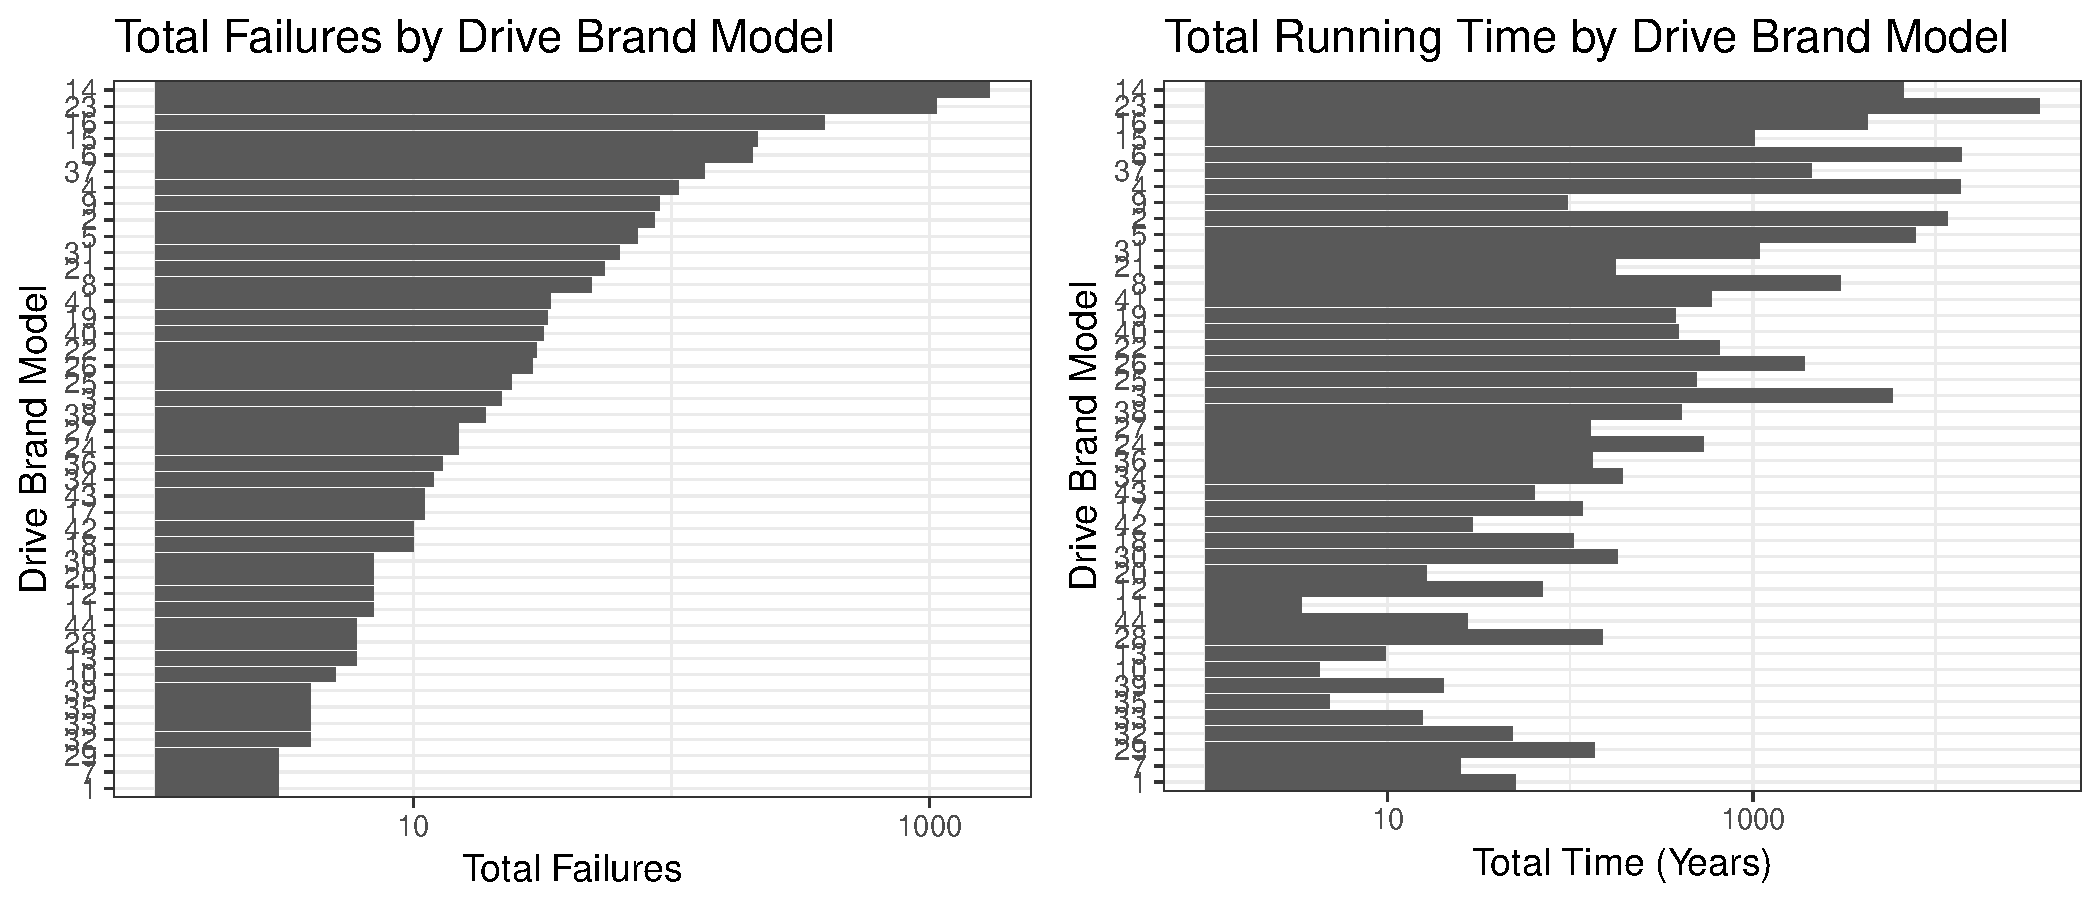
\includegraphics[width=.9\textwidth]{data-sum.pdf}
  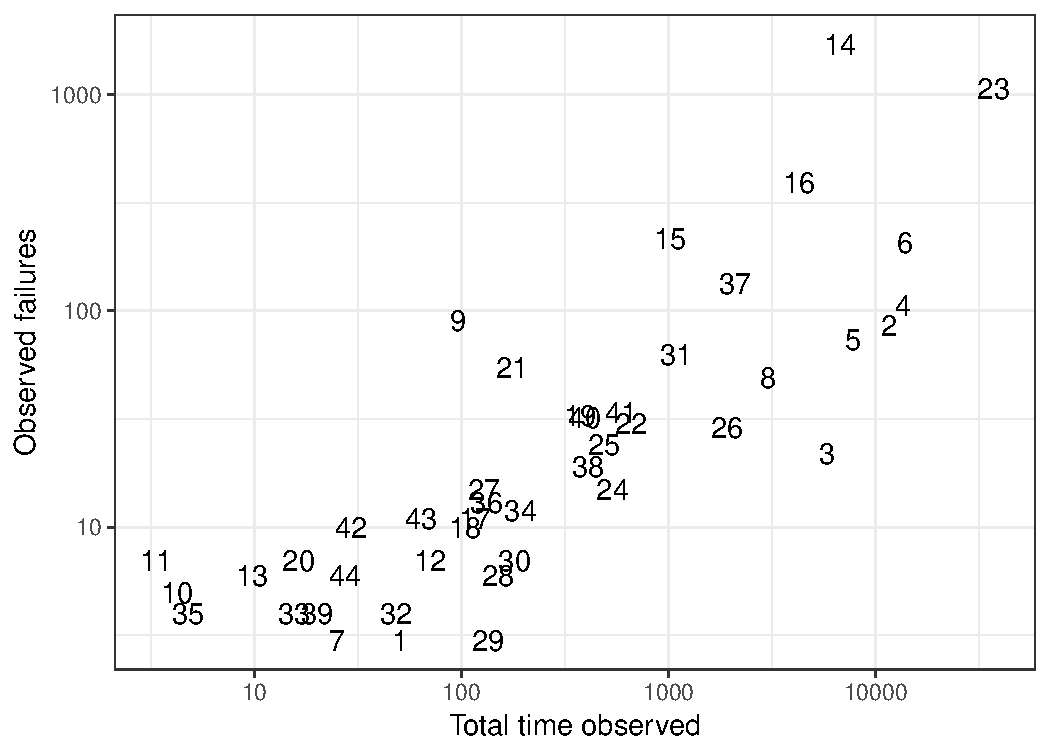
\includegraphics[width=.9\textwidth]{dm-summ-scatter.pdf}
  \caption{\footnotesize Scatterplot of total observed running time (hundred thousands of hours) versus total number of observed failures.  Each number labels a unique drive-model, numbered between 1 and 44.   Axes are on the log scale.}
  \label{drive-scatter}
\end{figure}

\subsection{Analysis of a single drive-model}
\label{subsec:ex1}
To illustrate the GLFP model, we will present an analysis of the drive-model with the most observed failures, Drive-model 14.  The Kaplan-Meier (K-M) estimate plotted below suggests at least two failure modes.  The curve has a slow ramp up in failures until about 10,000 hours (early failures), and increases more rapidly from about 10,000 to 20,000 hours (presumably wearout failures).  Besides our empirical observation, it is well known that computer hard drives have a mixture of early and late failures \citep{chan}.  Therefore, there is both an empirical and a theoretical justification to use the GLFP model in this application.

\begin{figure}[H]
\centering
  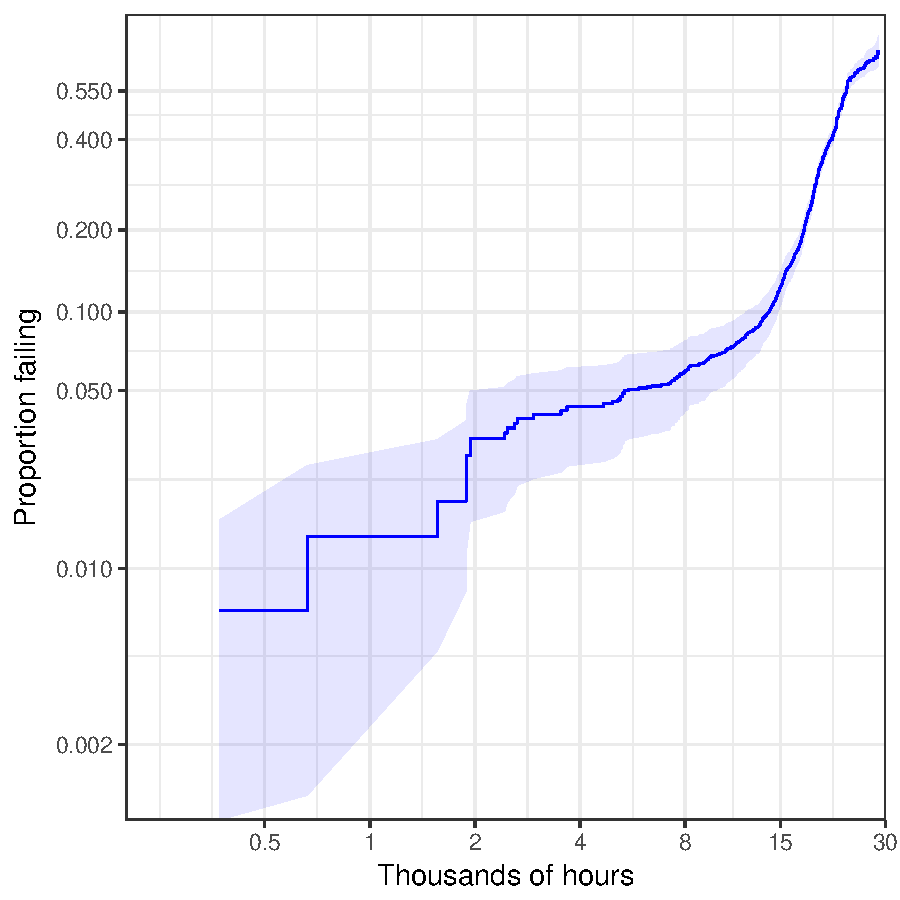
\includegraphics[width=.6\textwidth]{km14-prob}
  \caption{\footnotesize K-M estimate for Drive-model 14.  Uncertainty band correspond to pointwise standard errors (using Greenwood's formula.)}
  \label{fig1}
\end{figure}


To estimate the parameters of the GLFP model we use a Bayesian approach, selecting proper, but generally diffuse, prior distributions to improve identification of the model parameters. Having a proper prior distribution also ensures a proper posterior distribution. We reparameterize the component Weibull distributions using the $0.50$ quantile for the early failure mode ($t_{0.5,1}$) and the $0.20$ quantile for the wearout failure mode ($t_{0.2,2}$). \\

When eliciting prior distribution information it is much easier to ask about recognizable characteristics of a distribution instead of the traditional parameters of the distribution.  Following the approach used in \cite[Section 15.2.2]{intervals} we will use diagonal braces ($\langle.,.\rangle$) to refer to $95$ percent central probability intervals, rather than the standard model parameters when specifying prior distributions (See the Supplementary Material for standard density plots of the priors).  Using this convention the prior distributions used in our analyses are
%$$t_{0.5,1} \sim \op{Lognormal}(8,4), \quad t_{0.2,2} \sim \op{Lognormal}(10,4)$$
$$t_{0.5,1} \sim \op{Lognormal} \langle 1.7,\,7.6\times 10^6 \rangle,\quad
t_{0.2,2} \sim \op{Lognormal}\langle 8.6, \, 5.6\times 10^7 \rangle$$
$$\pi \sim \op{Logit-normal}\langle 0.001,\, 0.71 \rangle,\quad
\sigma_1, \sigma_2 \stackrel{ind.}{\sim} \op{Lognormal}\langle 0.0074 ,\,130 \rangle. $$
%\quad \sigma_2 \sim \op{Lognormal}\langle 7.4 \times 10 ^{-3} ,1.3 \times 10^2  \rangle $$

\noindent These prior distributions put probability mass on a wide range of values for all model parameters --- much larger than we would expect for a typical Weibull distribution.  Thus, these prior distributions are relatively uninformative. 


Table \ref{table:1} gives the posterior median and 95\% credible intervals for the 5 GLFP parameters for Drive-model 14.  The parameter $\pi$ is an estimate of the proportion of drives susceptible to early failure.  As expected, this proportion is small with a median value of 0.05.  The shape parameter estimates for the two Weibull distributions also match intuition.  The early failure mode puts posterior probability on a values of $\beta_1$ less than 1, which corresponds to a decreasing hazard.  Conversely, the credible interval for $\beta_2$, the wearout mode, is strictly above 1, implying an increasing hazard function.  The two quantiles are also well identified with the early failure mode having an much earlier time to reach the 0.50 quantile compared to the time to reach the 0.20 quantile for the wearout mode. 

\begin{table}[H]
\centering
\begin{tabular}{lrrr}
  \hline
 & Lower & Estimate & Upper \\ 
  \hline
$\pi$ & 0.033 & 0.054 & 0.099 \\ 
 $\beta_1 = 1/\sigma_1 $ & 0.47 & 1.13 & 1.72 \\ 
  $\beta_2 = 1/\sigma_2$ & 4.47 & 4.70 & 4.95 \\ 
  $t_{0.5,1}$ & $1.03$  & $2.28$ & $3.99$\\ 
  $t_{0.2,2}$ & $18.0$ & $18.2$ & $18.6$ \\ 
   \hline
\end{tabular}
\caption{\footnotesize Posterior 95\% Credible Intervals for the 5 GLFP parameters for Drive-model 14.  The quantiles are in thousands of hours.}
\label{table:1}
\end{table}


Probability plotting is a simple method to assess and compare the adequacy of members of the log-location-scale family of distributions.  After properly transforming the axes of a plot, graphing an empirical estimate of fraction failing as a function of time along with confidence bands provides a visual assessment of distributional goodness of fit.  We applied this method using the Kaplan-Meier nonparametric estimate of the empirical cdf.  With left truncation, however, the standard Kaplan-Meier estimator is biased, so we used an adjusted version due to \citet[Chapter 11]{meeker} (see Appendix for a detailed description).   


In Figure \ref{ex1-overlay}, we overlay the posterior median of the fitted GLFP model onto the adjusted K-M estimate with axes on the Weibull probability scale.  The plot also contains 90\% pointwise credible bands associated with each estimate. While the Weibull model is inadequate for these data, the GLFP model fits quite well, as it is able to adequately describe the rapid increase in the empirical cdf between 8000 and 20,000 hours. %The discrepancy around 30,000 suggests that the GLFP may overestimate the proportion failing in the far right tail of the distribution.  While this discrepancy may appear troubling, we suggest that the right tail is of less importance for electronic goods due to obsolescence.

\begin{figure}[H]
\centering
  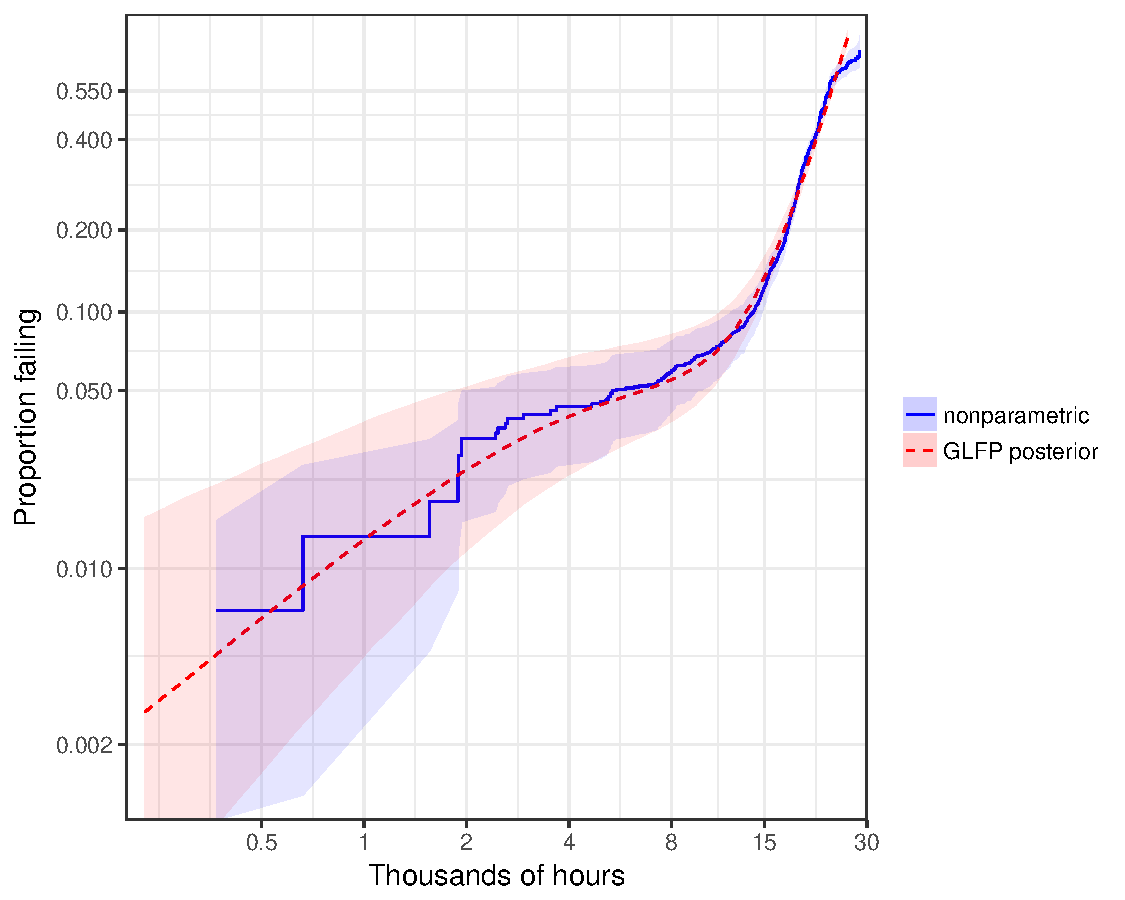
\includegraphics[width=.8\textwidth]{km14-prob-plus}
  \caption{\footnotesize The estimated GLFP model for Drive-model 14 plotted on Weibull paper.  The dashed line corresponds to the median of the posterior draws; pointwise 90\% credible bounds are indicated by the smooth region.  The solid line is an adjusted K-M estimate with pointwise 90\% credible bounds in blue.}
  \label{ex1-overlay}
\end{figure}


\section{Hierarchical GLFP model}
\label{sec:Hierarchical GLFP model}
In order to describe an entire product population, consisting of different but similar sub-populations, and because of the limited amount of data from many of the sub-populations, we model sub-population-specific parameters hierarchically, borrowing strength across sub-populations.

\subsection{Conditional likelihood}
Let
\begin{equation}
T_{ig} \ind \op{GLFP}\left( \pi_g, t_{p_{1}g}, \sigma_{1g}, t_{p_{2}g}, \sigma_{2g} \right),
\end{equation}
where $g=1,\ldots,G$ indexes the sub-populations.  The likelihood for the GLFP model for all subpopulations is a function of the sets of parameters $\bm{\theta_g} = (\pi_{g}, t_{p_{1}g}, \sigma_{1g}, t_{p_{2}g}, \sigma_{2g})$, one set for each sub-population, $g$.  Assuming the lifetimes of all units are independent within and across sub-populations, and conditional on fixed values of the parameters, the likelihood for the data, $i=1,\dots,n_g$,  is given by
\begin{equation*}
L(\bm{\Theta})= \prod_{g=1}^{G} \prod_{i=1}^{n_{g}} \left[\frac{h(t_{ig};\bm{\theta_g})}{1-H(t_{ig}^L;\bm{\theta_g})}\right]^{1-c_{ig}} \left[ \frac{1-H(t_{ig};\bm{\theta_g})}{1-H(t_{ig}^L;\bm{\theta_g})} \right]^{c_{ig}}
\end{equation*}
where $T_{ig}$ is the observed failure or survival time of unit $i$ in sub-population $g$; $t_{ig}^L$ is the left truncation time for unit $i$ in sub-population $g$; and $c_{ig}$ is an indicator if unit $i$ in sub-population $g$ is right censored. All times are in thousands of hours.  Again, this likelihood
is easy to modify for other situations like interval-censoring,
as explained in Section~\ref{subsec:likehood}.

\subsection{Parameter distributions}

In a hierarchical model, the parameters are modeled as random variables, varying across different sub-populations.  For example
\begin{equation*}
\sigma_{1g} \ind \op{Lognormal} \left( \eta_{\sigma_1}, \tau^2_{\sigma_1} \right)
\end{equation*}
\begin{equation*}
\sigma_{2g} \ind \op{Lognormal} \left( \eta_{\sigma_2}, \tau^2_{\sigma_2}\right)\op{Tr}\left(0, 1\right)
\end{equation*}
\begin{equation}
\label{eq:hier-model}
t_{p_{1}g} = \exp\left(\mu_{1g} + \sigma_{1g}\,\Phi^{-1}(p_1)\right)  \ind \op{Lognormal} \left(\eta_{t_{p_1}}, \tau^2_{t_{p_1}}\right)
\end{equation}
\begin{equation*}
t_{p_{2}g} = \exp\left(\mu_{2g} + \sigma_{2g}\,\Phi^{-1}(p_2)\right)  \ind \op{Lognormal} \left(\eta_{t_{p_2}}, \tau^2_{t_{p_2}}\right)
\end{equation*}
\begin{equation*}
\pi_g \ind \op{Logit-normal}(\eta_\pi, \tau^2_\pi).
\end{equation*}

As discussed in Section \ref{sec:Weibull parameterization}, we reparameterize the Weibull distribution in terms of a quantile and the shape parameter because observed failure data are often more informative about the lower tail of their respective lifetime distribution (note that if $T$ has a Weibull distribution, $\sigma$ is a shape parameter for the distribution of $T$ and a scale parameter for the distribution of $\log(T)$). We truncate the distribution of $\sigma_{2g}$ at $1$ (indicated by $\text{Tr}(0,1)$ above) restricting the wearout failure mode to have an increasing hazard function (i.e., $\beta_{2g} = 1/\sigma_{2g}>1$). %We choose to model these parameters with log-normal and logit-normal distributions because many populations require strong regularization which the normal, with its exponentially decreasing tails, provides. 

\subsection{Prior Distributions}
The complete GLFP model requires prior distributions on the hierarchical parameters.  We suggest weakly informative proper distributions that allow the data to overwhelm the prior distribution and provide information about the distribution of the population parameters.  Prior knowledge about product lifetimes is useful for choosing the mean of the location parameter ($\eta$) distributions.  However, the corresponding standard deviations should be diffuse to allow the location to vary depending on the observed data.  For the scale parameters ($\tau$) we use half-Cauchy distributions as suggested by \citet{gelman2014bayesian}.  

\subsection{Nested models}
In principle, we prefer the full model (\ref{eq:hier-model}) because we tend to believe that every population has a distribution with a distinct set of parameters. In practice, however, we may consider restrictions to reduce the number of parameters if the data do not support their inclusion.  We considered four models, all based on (\ref{eq:hier-model}), differing by which model parameters are held constant across sub-populations. These are (from most to least restrictive):

\paragraph{Model 1} $\pi_{g} = \pi,\quad t_{p_{1}g} = t_{p_1},\quad \sigma_{1g}=\sigma_1,\quad t_{p_{2}g} = t_{p_2},\quad \sigma_{2g} = \sigma_2$
\paragraph{Model 2} $\pi_{g} = \pi,\quad t_{p_{1}g} = t_{p_1},\quad \sigma_{1g}=\sigma_1,\quad \sigma_{2g} = \sigma_2$
\paragraph{Model 3} $\pi_{g} = \pi,\quad  t_{p_{1}g}= t_{p_1},\quad \sigma_{1g}=\sigma_1$
\paragraph{Model 4} $t_{p_{1}g}= t_{p_1},\quad \sigma_{1g}=\sigma_1$


This set of model specifications is chosen based on the data, interpretation of the model, as well as estimation considerations.  Sub-population-model-specific parameters for the the wearout failure mode $(t_{p_{2}g},\sigma_{2g})$, and the proportion defective $(\pi_g)$, are considered as a means to account for heterogeneity across sub-populations in the right tails of the lifetime distribution.  Going from a common model for all sub-populations and gradually increasing the complexity of the model, Model 4 is the most flexible.  Model 4 allows for the probability of early failure as well as the shape and scale parameters for the wearout failure mode to vary across sub-populations.

For all of the nested models, the parameters for the early failure mode are common across sub-populations.  We found that there was often insufficient information to model these parameters hierarchically.  Moreover, assuming a common distribution for early failures provides a meaningful interpretation and comparison of the $\pi_g$ across the subpopulations.  Also the lifetime distribution of the defective subpopulation (as opposed to the proportion defective) is not of high interest.

\subsection{Model selection}
The use of Bayes factors is a classical apporach to compare alternative model specifications.  However, they can be problematic, especially in high dimensional settings where there is no concensus on how to properly compute the required marginal likelihood \citep{robert2016}. Moreover, from the point of view of a consumer or purchaser, the goal of an analysis such as this is to rate manufacturers and/or to inform future purchases based on predicted product performance. Therefore, we should compare model specifications based on accurate prediction for future units of previously observed products.  Leave-one-out cross-validation (LOO) is a method to estimate out-of-sample predictive accuracy using
posterior draws from a fitted model.  Following \cite{vehtari}, the log pointwise predictive density (lpd), is one method to quantify predictive accuracy,

\begin{align*}
\mbox{lpd} &= \sum_{g=1}^G \sum_{i=1}^{n_g} \log[p(t_{new,g,i}|t, t^L, c)] \\
&= \sum_{g=1}^G \sum_{i=1}^{n_g} \log \left[ \int p(t_{new,g, i}|\theta) p(\theta|t,t^L,c) d\theta \right].
\end{align*}
\noindent Using this criterion, we should choose the model with the highest expected lpd (elpd) for a new data set $\{t_{new,g,i}:g=1,\ldots,G; i=1,\ldots,n_g\}$. Notationally suppressing the conditioning on $t^L$ and $c$,
\begin{equation}
\mbox{elpd} = \op{E}_h \mbox{lpd} = \sum_{g=1}^G \sum_{i=1}^{n_g} \int \log [p(t_{new, g, i}|t)] h(t_{new,g,i}) d t_{new,g,i}
\label{elpd}
\end{equation}
where $h$ is a density for the true distribution of $t_{new,g,i}$. Although $h$ is unknown, leave-one-out cross-validation provides a robust estimator:
\begin{equation}
\widehat{\text{elpd}} = \sum_{g=1}^G \sum_{i=1}^{n_g} \log [p(t_{g,i}|t_{-(g,i)})].
\label{loo-est}
\end{equation}
The \texttt{R} package, \texttt{loo} \citep{loo}, computes an approximation of (\ref{loo-est}) provided that the observations $t_i$ are conditionally independent. It employs an importance sampling method that uses $S$ saved MCMC draws to compute smoothed importance weights, $w_{i,s}$, approximating $p(t_{g,i}|t_{-(g,i)})$ with $\sum_{s=1}^S w_{i,s} p(t_{g,i})/\sum_{s=1}^S w_{i,s}$. In addition to providing an estimate of (\ref{elpd}), their method also produces a standard error based on an asymptotic result.  A measure of the effective number of parameters is also available using the sum of the posterior variance of the log predictive density for each observation.
%When $n$ is large, the distribution of the elpd is approximately normal and different models can be compared statistically. 
% To statistically compare the GLFP Models, we estimated the predictive accuracy of the 4 different models using an approximate leave-one-out cross validation (LOO) method.  As outlined in Vehtari et. al, the predictive accuracy from a fitted Bayesian model can be estimated simply with posterior draws of the model parameters rather than re-fitting the model with different data sets \cite{vehtari}.  For each observation, $i$, the log point-wise predictive density is calculated over the full set of posterior samples with data point $i$ removed.  
% The final expected log point-wise predictive density (elpd) is the sum over all observations (elpd $=\sum{\log p(y_i|y_{-i})}$).  

\section{Model for the Backblaze hard drive data}
\label{sec:Data analysis}
We now apply this general methodology to the hard drive failure data from Backblaze.  There are 44 different drive-models in the data set, and significant heterogeneity in the number of observed failures, time observed (Figure 1), and the parameter estimates of the underlying GLFP model. The hierarchical GLFP model allows us to describe the entire drive-model population, borrowing information across drive-models, allowing estimation for those drive-models for which there is little information (i.e., few failures). 

\subsection{Prior distributions}
\label{sec:Prior distributions}
Following the recommendations in Section 5.3, we specify the following prior distributions for each of the four nested GLFP models. Different sets of restrictions require different prior distribution specifications, which are assigned as follows:

\paragraph{Model 1} Constrain all drive-models to the same GLFP distribution. For this ``reduced" model we assume the same prior distributions as in Section \ref{subsec:ex1}.

\paragraph{Model 2} $t_{p_{2}g}$ varies by drive-model. To help with model identifiably, we tighten the priors on the early failure mode:
$$ \pi \sim \op{Logit-normal}\langle 0.007,\, 0.26 \rangle,$$
$$\sigma_1 \sim \op{Lognormal}\langle 0.14,\, 7.1\rangle,$$ 
$$t_{0.5} \sim \op{Lognormal} \langle 22,\, 5.5 \times 10^{4} \rangle.$$

\paragraph{Model 3} $t_{p_{2}g}$ and $\sigma_{2g}$ vary by drive-model. Prior distributions for the constrained parameters are the same as for Model 2.

\paragraph{Model 4} $\pi_g$, $t_{p_{2}g}$ and $\sigma_{2g}$ vary by drive-model. Prior distributions for constrained parameters are the same as for Model 2.


Where applicable, prior distributions on hyperparameters are as listed below. We use half-Cauchy prior distributions on hierarchical scale parameters. As for the location hyperparameters, we choose weakly informative prior distributions centered around the corresponding prior mean for the non-hierarchical model.
$$\eta_{\pi} \sim \op{Normal}(-3, 1^2),\quad \tau_{\pi} \sim \op{Half-Cauchy}(0, 1)$$
$$\eta_{\sigma_2}  \sim \op{Normal}(0, 2^2),\quad
\tau_{\sigma_2}  \sim \op{Half-Cauchy}(0, 1)$$
$$\eta_{t_{0.2}}  \sim \op{Normal}(9, 2^2),\quad
\tau_{t_{0.2}}  \sim \op{Half-Cauchy}(0, 1).$$

\subsection{Model fitting}
\label{sec:Model fitting}
Each model was fit using the {\tt
  rstan} \citep{rstan} package in {\tt R} \citep{r}, which implements a variant of Hamiltonian Monte Carlo (HMC)
\citep{betancourt}. HMC jointly updates all model parameters by simulating energy preserving paths with random initial momentums along the posterior density. This is done to reduce autocorrelation and efficiently explore the posterior. Multiple chains were run, each with 1500 iterations after 1500 warmup iterations: 4 chains were run for Models 1, 2 and 3 for a total of 6,000 post burn-in iterations and 16 chains were run for Model 4 for a total of 24,000 post burn-in iterations. The Gelman-Rubin potential scale reduction factor was used to provide a check for adequate mixing of the multiple chains. Upon convergence, $\hat{R}$, converges to 1.  The  respective maximum values of $\hat{R}$ across all model parameters for Models 1 through 4 (5, 50, 95 and 140 parameters, respectively) were 1.005, 1.028, 1.009 and 1.004. Other diagnostics provided by the software (tree-depth, and divergent transitions) did not indicate problems with sampling. Plots of the posterior draws were inspected for parameters with the smallest effective sample size; these did not suggest features that were inadequately explored.



\subsection{Model selection}
\label{sec:Model Comparisons}
As we have discussed, while we would prefer to allow all of the GLFP model parameters to be drive-model specific, there are practical issues with fitting the full model. For example, due to heavy left-truncation, there may be insufficient information for particular drive-models to estimate all of the parameters. 

Figure \ref{fig:fig2} provides a visual comparison for Models 1 through 4 by plotting the pointwise posterior median of the cdf for each drive-model.  The large left panel shows the adjusted K-M estimate.  The smaller plots correspond to Models 1 through 4.  To make the plots comparable, we use an adjustment based on the parametric model (Model 4).  Note that while all the paths for the posterior estimates necessarily pass through the origin, the K-M estimates do not, because, for the K-M estimator, inference is entirely conditional on survival up to left-most left-trunctation time.

%Should we be brief discussing the plot?
These plots suggest that Model 1 is insufficient to explain the observed data. Model 2 certainly captures more of the heterogeneity observed in the K-M estimates; we observe that the assumption of a common $\sigma_2$ results in similar progressions in the cdf, which may be too restrictive. Model 3, which allows $\sigma_2$ to vary by sub-population, suggests there is evidence to support variation in this parameter among drive-models. While there are differences between Model 3 and 4, they are relatively subtle.

\begin{figure}[H]
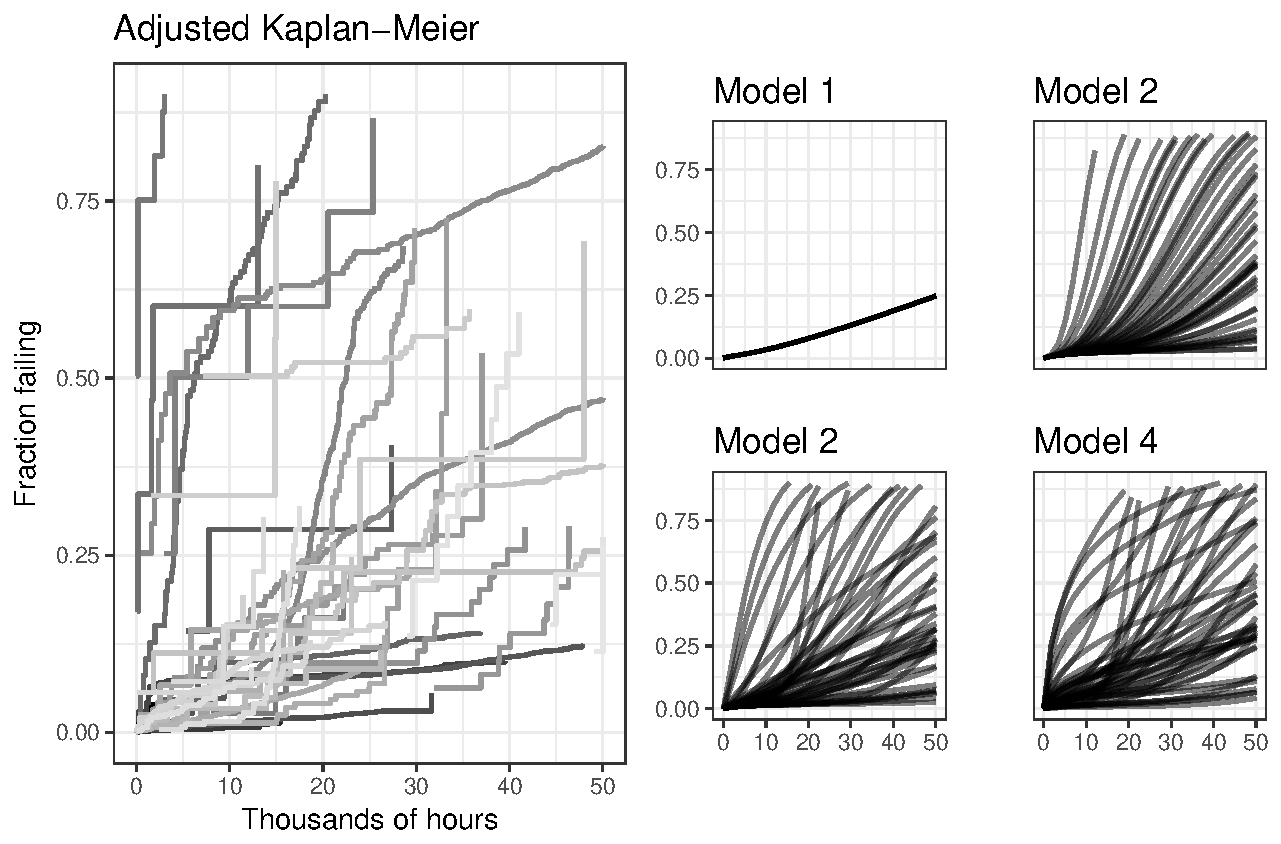
\includegraphics[width=\textwidth]{heterogeneity-compare}
\caption{\footnotesize Left: Adjusted K-M estimates of the time to failure for each of the drive-models in the Backblaze data. Right: Pointwise posterior median cdf estimates for Models 1-4, ordered left to right, top to bottom.}
\label{fig:fig2}
\end{figure}

We can also compare posterior estimates of time to failure under Models 1-4 for each drive-model individually.  For these comparisons we calculate pointwise the posterior median of the proportion failing over a grid. That is, for every model, and for a fixed set, $\tilde{t}=\{\tilde{t}_1,\ldots,\tilde{t}_M\}$, we compute 
\begin{equation}
\label{pointwise-medians}
\op{median}\left\{\op{H}\left(\tilde{t}_m|\pi_{g}^{(s)},t_{p_{1}g}^{(s)},\sigma_{1g}^{(s)},t_{p_{2}g}^{(s)},\sigma_{2g}^{(s)}\right);s=1,\ldots,S \right\},
\end{equation}
where $\theta^{(s)}$ is posterior sample $s$ from $p(\theta|y)$.
%Unlike maximum likelihood, by including the hyperparameters in the probability model, there is a data-dependent penalization that results in shrinkage toward a common overall model.

\begin{figure}[H]
{\centering
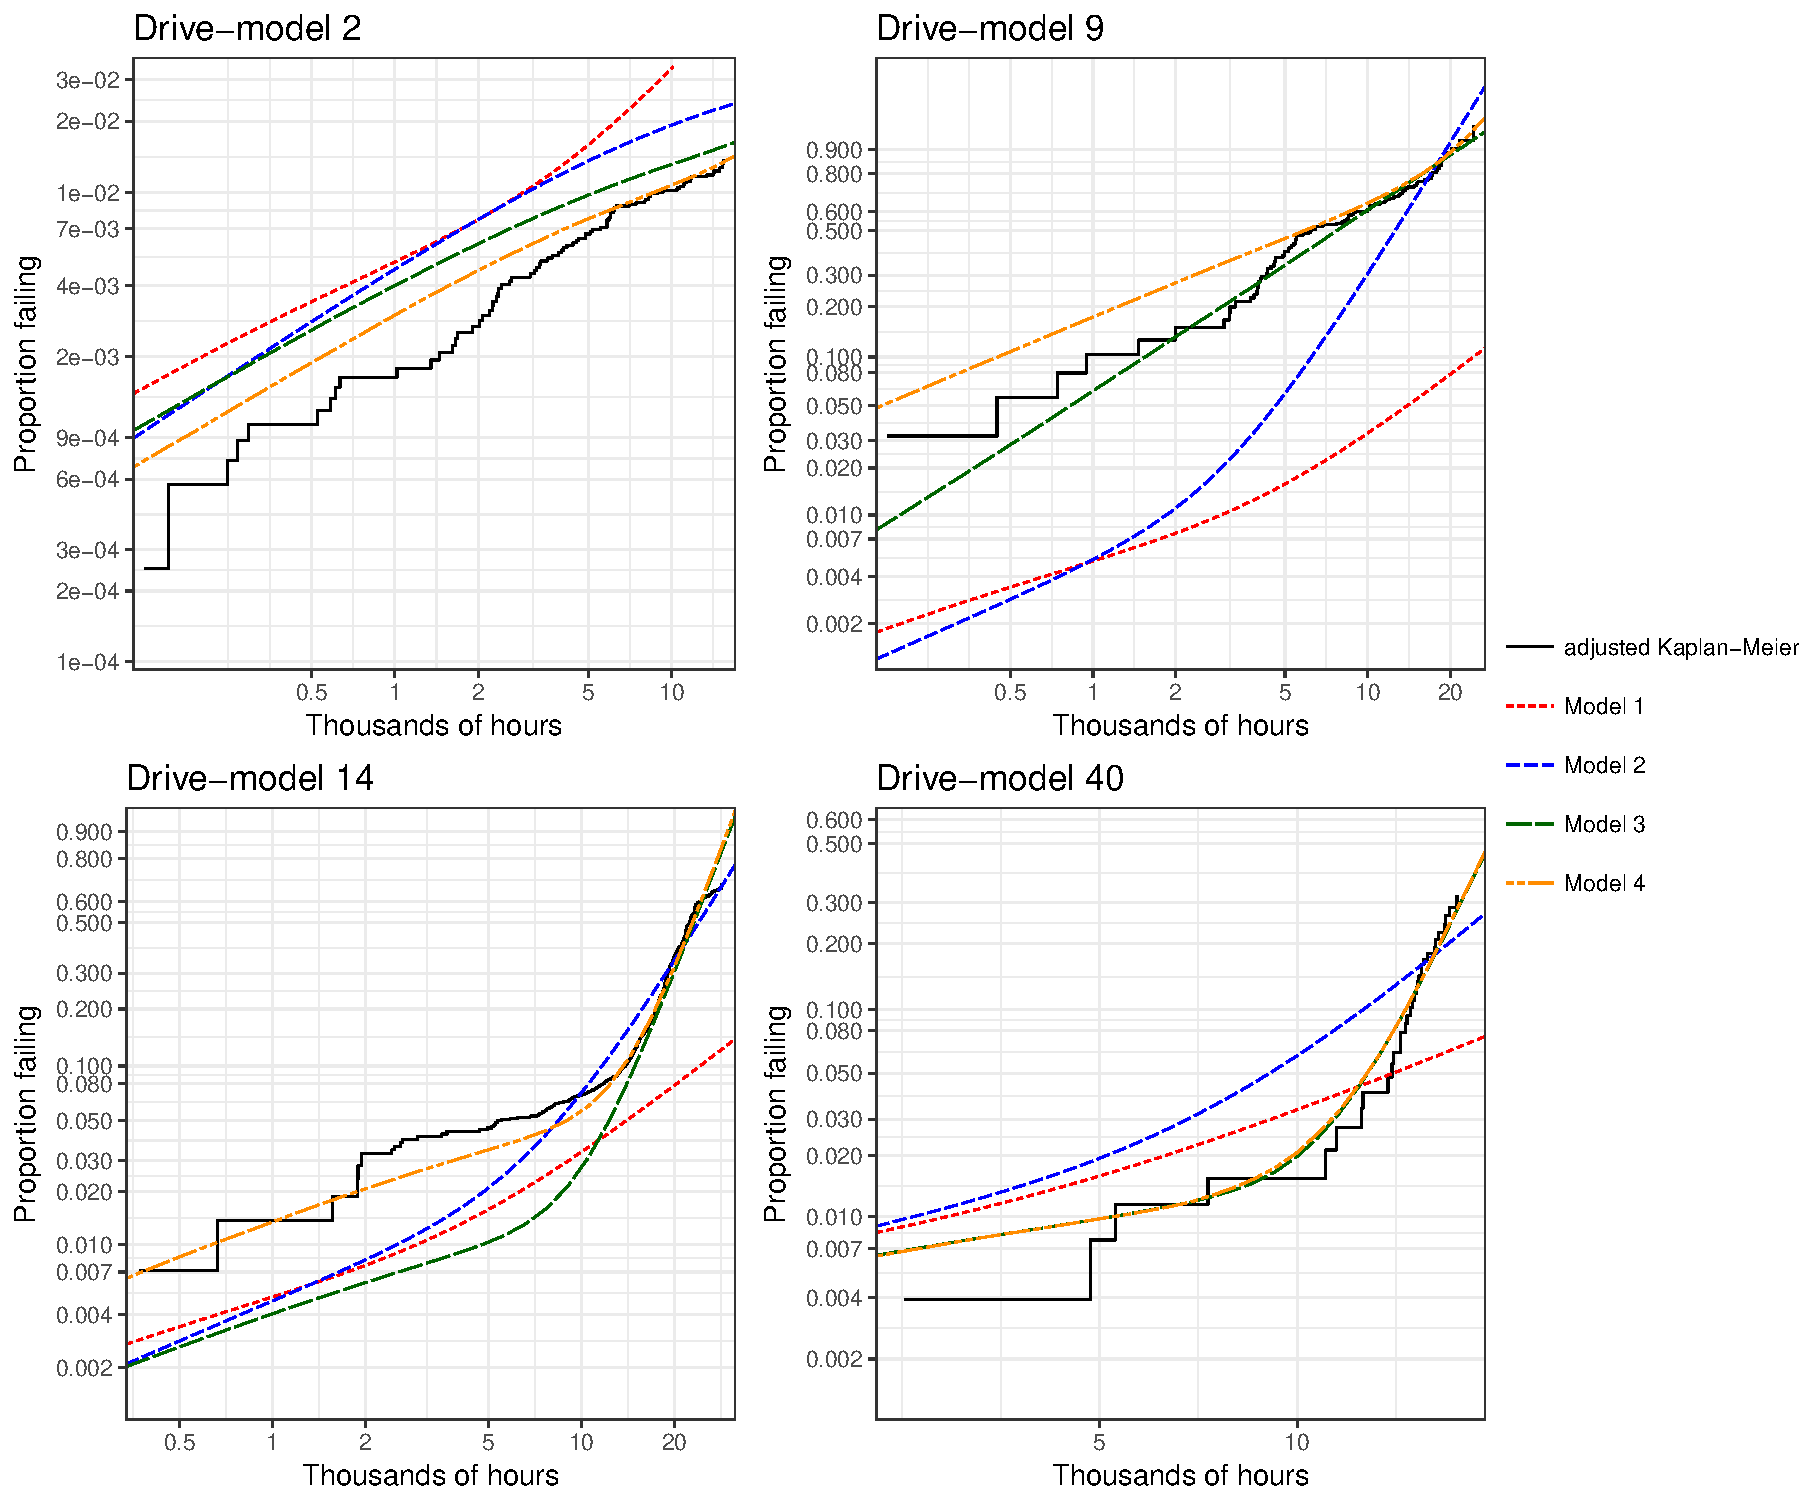
\includegraphics[width=\textwidth]{single-drive-4-Models-ex-v2}}
\caption{\footnotesize Posterior median of the proportion failing as a function of time under Models 1-4 for sample of drive-models, with axes scales as for Weibull probability plotting.  The solid step function is the adjusted K-M estimate.}
\label{fig:mod_comp_leg}
\end{figure}

%stopped here
The GLFP model fits for a representative selection of drive-models (Drive-models 2, 9, 14, and 40) are presented in Figure \ref{fig:mod_comp_leg} (See the Supplementary Material for similar plots for the other drive-models).  The step functions again correspond to the adjusted K-M estimates.  As model complexity increases, the hierarchical-model GLFP curves become more flexible and are better able to describe the observed failure data.  All of the GLFP models appear to produce higher estimates of the proportion failing, relative to K-M, for Drive-model 2. This behavior is not unexpected, however, because hierarchical models improve model stability through shrinkage; in this context, shrinkage is toward an average cdf. Model 4 is in closest agreement. 

Drive-model 9 shows a high proportion of early failures, a fact which Model 1 fails to capture. Model 2 addresses this by estimating an earlier time to wearout, but still results in a poor fit to the data. Models 3 and 4 conform more closely to the adjusted K-M estimate. The disagreement between Models 3 and 4 for Drive-model 9, is interesting: Model 4 allows the proportion of defective units to vary by drive-model, but Model 3 appears to fit just as well in this case, by increasing the scale parameter for the wearout failure mode.

For Drive-model 14, Models 1-3 produce lower estimates of the proportion of drives failing, and for Drive-model 40, they produce higher estimates.  On the other hand, Model 4 follows the K-M closely across both stages of lifetime.  The differences between Models 3 and 4 and Models 1 and 2 are visually apparent.  Differentiating between Model 3 and 4 is less clear; for instance, the estimates from Model 3 and 4 are nearly identical for Drive-model 40.


Results showing the estimated elpd and associated standard errors for all 4 models are shown in Table \ref{table:2}.
We calculated the difference in expected predictive accuracy for Model 4 versus 3, Model 3 versus 2, and Model 2 versus 1, as well as the standard error of the difference (Table 2). For the models we considered, each successive increase in model complexity increases the elpd.  Of all the models, Model 4 has significantly better elpd compared to the the other 3 models.

\begin{figure}
\begin{table}[H]
\centering
\begin{tabular}{rrrrrrrr}
  \hline
 & $\widehat{\text{elpd}}$ \ & \thead{Estimated Difference \\ in $\widehat{\text{elpd}}$} \ & \thead{Standard Error of \\ the Difference} & \thead{Effective Number of \\ Parameters}\\ 
  \hline
Model 4 & -13309.5 & 40.7 & 11.3 & 92.5 \\ 
Model 3 & -13350.2 & 458.8 & 31.0 & 68.8 \\ 
Model 2 & -13809.0 & 3674.6 & 96.2 & 49.6 \\ 
Model 1 & -17483.6 &  &  & 4.3 \\
   \hline
\end{tabular}
\caption{\footnotesize Expected log pointwise predictive density (elpd) and related statistics for each model.}
\label{table:2}
\end{table}
\end{figure}

\section{Model Assessment}
\subsection{A simulation-based approach}
\label{model-assessment}
Having selected a model, it is good practice to check that the model provides an adequate representation of the data-generating mechanism. One way to do this is to draw replicate data sets from the posterior predictive distribution
$$p(t_{rep,g}|t) = \int \prod_{i=1}^{n_g} f(t_{rep,g,i}|\theta_g)\; p(\theta_g|t)\;d\theta_g,$$
in the case that observations in subpopulation $g$ are exchangable.  This is approach is recommended by \cite{gelman1996postpred} in part because it works well in cases when no classical goodness-of-fit test is available. When the model is adequate for the data, the predictive distribution of a finite set of data characteristics --- chosen to reflect features relevant to the goals of the analysis --- should not contradict the corresponding characteristics observed in the actualized data.

There are many possible approaches to the posterior predictive check. We propose the comparison of K-M estimates for each sub-population derived from replicated data drawn from the posterior predictive distribution to the K-M estimate based on the actualized data. This graphical approach does not provide a test statistic, but provides rich feedback with respect to the fitted model's agreement with the data.

Because the variability in the K-M estimator is primarily a function of the number of at-risk units, we want to replicate the pattern of censoring that was observed. To do this, we sample from a version of the posterior predictive that conditions on the observed truncation and censoring times, i.e. 
$$p(t_{rep,g}|t) = \int \prod_{i=1}^{n_g}f(t_{rep,g,i}|t_{g,i}^L,c_{g,i},\theta_g)\;p(\theta_g|t)\;d\theta_g.$$

An obstacle remains, owing to the fact that the censoring time is unknown for observed failures. We resolve this by assuming that failed units would have been right censored had they survived until the latest censoring or failure time for that drive model.

Our method for generating replicate data sets, $t_{rep,g}^{(s)}$, $s = 1,\ldots, R$, for each sub-population $g=1,\ldots,G$, is as follows:

For $s=1,\ldots, R$,

\begin{enumerate}
\item Sample $r$ uniformly from $\{1,\ldots,S\}$.\\ For $i=1,\ldots,n_g$, do:
\item Simulate $\tilde{t}_{rep,g,i}^{(s)} \sim \op{GLFP}(\pi_{g}^{(r)},t_{p1}^{(r)},\sigma_1^{(r)},t_{p_{2}g}^{(r)}, \sigma_{2g}^{(r)}).$
\item Repeat step 2 until $\tilde{t}_{rep,g,i} > t_{g,i}^L$
\item Set $d_{g,i}^{(s)}= \begin{cases} \max \{t_{g,i}: i \ge 1\}, & \mbox{ if }c_{g,i}=0\\
t_{g,i}, & \mbox{ if }c_{g, i}=1. \end{cases}$\\
Lastly, set $(t_{rep,g,i}^{(s)},c_{rep,g,i}^{(s)}) = \begin{cases}
  (d_{g,i}^{(s)},1), & \mbox{ if } \tilde{t}_{rep,g,i}^{(s)}>d_{g,i}^{(s)}\\
  (\tilde{t}_{rep,g,i}^{(s)},0), & \mbox{ if }\tilde{t}_{rep,g,i}^{(s)} \le d_{g,i}^{(s)}.
\end{cases}$
\end{enumerate}
Finally, plot K-M estimates based on the $R$ replicated data sets along with the one based on the observed data on the same axes. Discrepancies between the replicated and actual data can be used to diagnose inadequacies of the model.

\subsection{Application to the Backblaze data}
For the hard-drive data, we used the posterior samples obtained in fitting Model 4 to generate $R=19$ replicate data sets as described above. The resulting plots for Drive-models 2, 9, 14, and 40 are displayed in Figure \ref{fig:post-pred-KM} (see the Supplementary Material for similar plots for all of the drive-models).



\begin{figure}
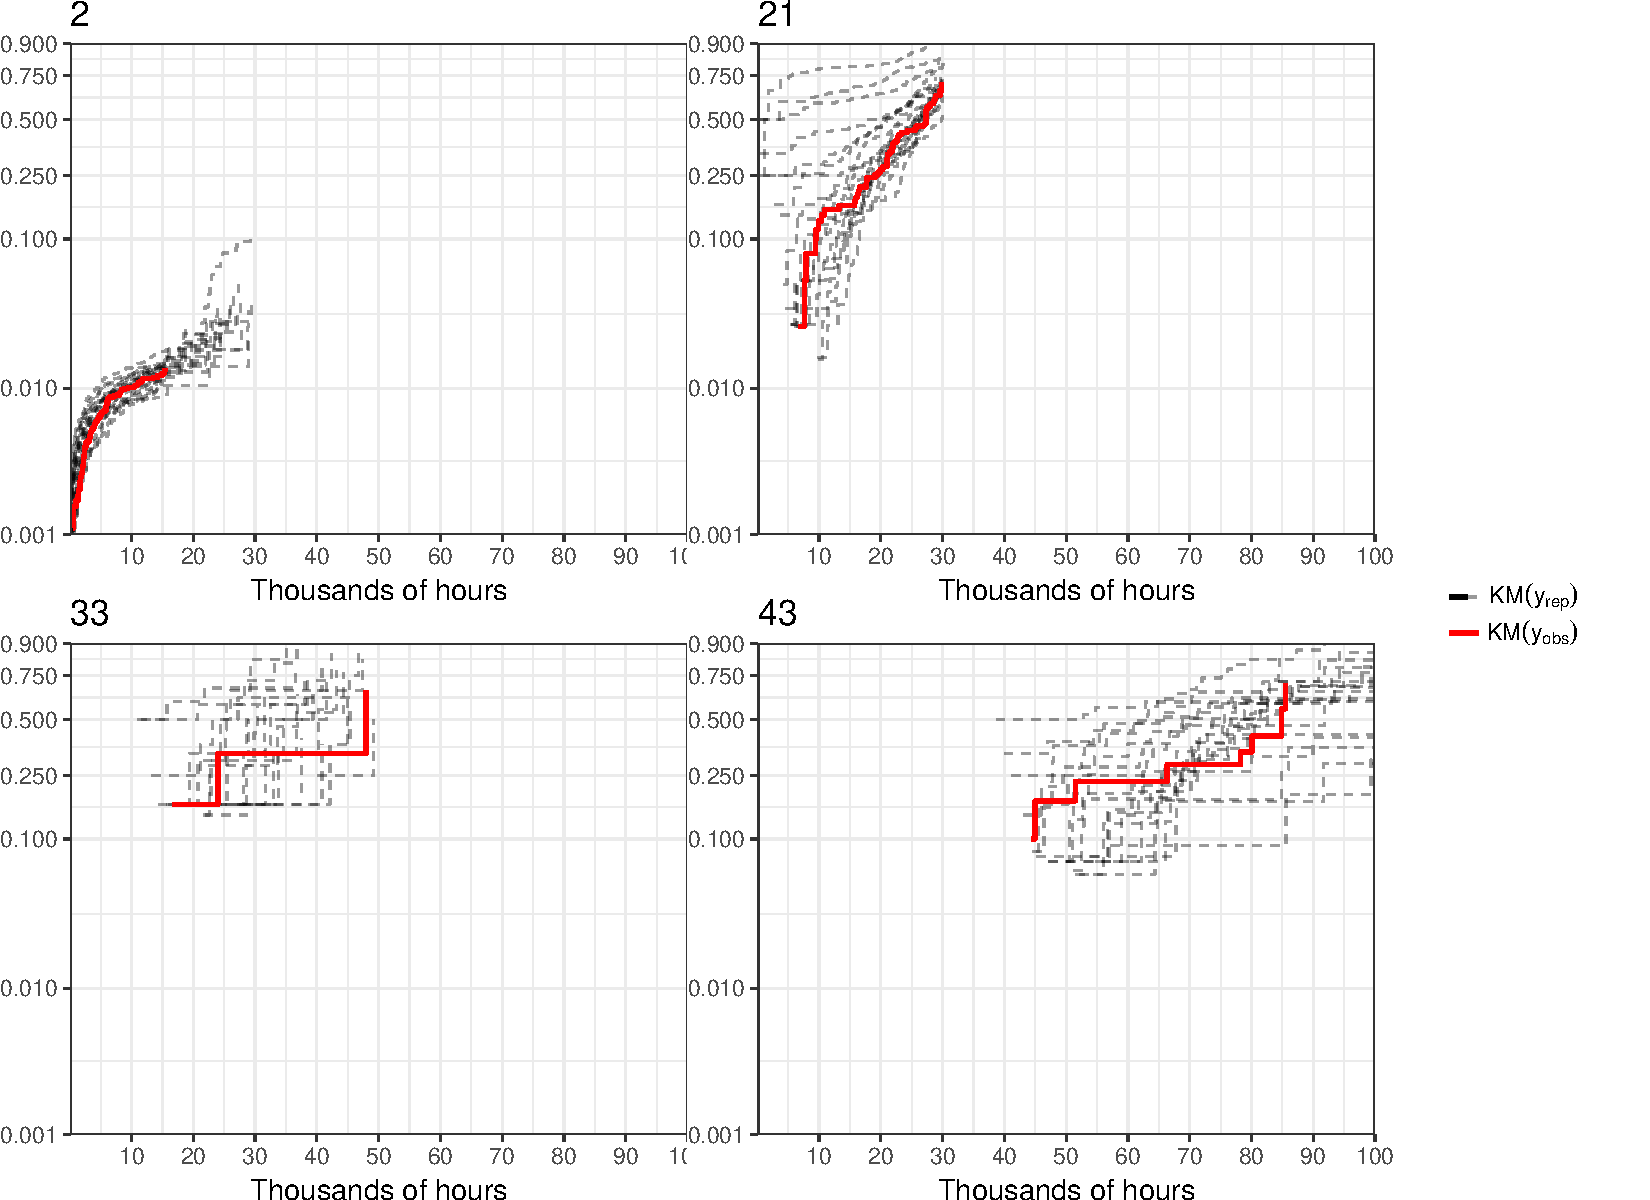
\includegraphics[width=\textwidth]{ppcheck-sample}
\caption{\footnotesize Adjusted K-M estimates of the proportion failing for a representative subset of drive-models. Both the original data (\textbf{bold} line) and 19 ``replicated" data sets from the posterior predictive distribution (\textit{dashed} lines) are shown.}
\label{fig:post-pred-KM}
\end{figure}

For most drive-models, the estimates based on the observed data look similar to those based on the replicated data.  There are a few drive-models, however where this is not the case. Drive-model 14 shows a discrepancy between the GFLP fit and the K-M fit in the right tail. In particular, the GLFP predictions appear conservative, overpredicting the proportion failing after about 2.5 years. Due to the large number of failures for this drive-model, the posterior for the hierarchical model is similar to the stand-alone model. Other drive-models showing a lack of fit are 4 and 34. We first address Drive-model 4; our diagnosis of 34 is analogous, so the following comments extend to that drive-model as well.


To diagnose the cause of the discrepancies between the observed data for Drive-model 4 and its posterior predictive distribution, we consider the event plot for a random sample of units for this Drive-model while looking at estimates of lifetime (Figure \ref{fig:ex-mod-4}). From these plots, we can see that the discrepancy between the posterior and K-M estimates is driven by failures among a relatively small subset of units, namely those with left-truncation times smaller than 2500 hours. Further investigation reveals that, if we exclude the newest 75 drives, those with truncation times less than 800 hours, the K-M estimate falls within the posterior 90\% pointwise credible band. This situation suggests that, despite belonging to the same drive-model, there may be something different about the newer drives leading to worse reliability. 

A possible explanation for the discrepancy shown in Figure 7 is that
the units of Drive-model 4 were introduced into the field over a
period of 22 months. Manufactures of hard drives (and most other
products) often make changes to the product design over time to
either improve reliability or to reduce cost. Such changes will
sometimes have an important effect on the product's lifetime
distribution, invalidating one of our important assumptions that
lifetime distribution for a drive-model does not depend on the
date of manufacture. 

\begin{figure}
\centering
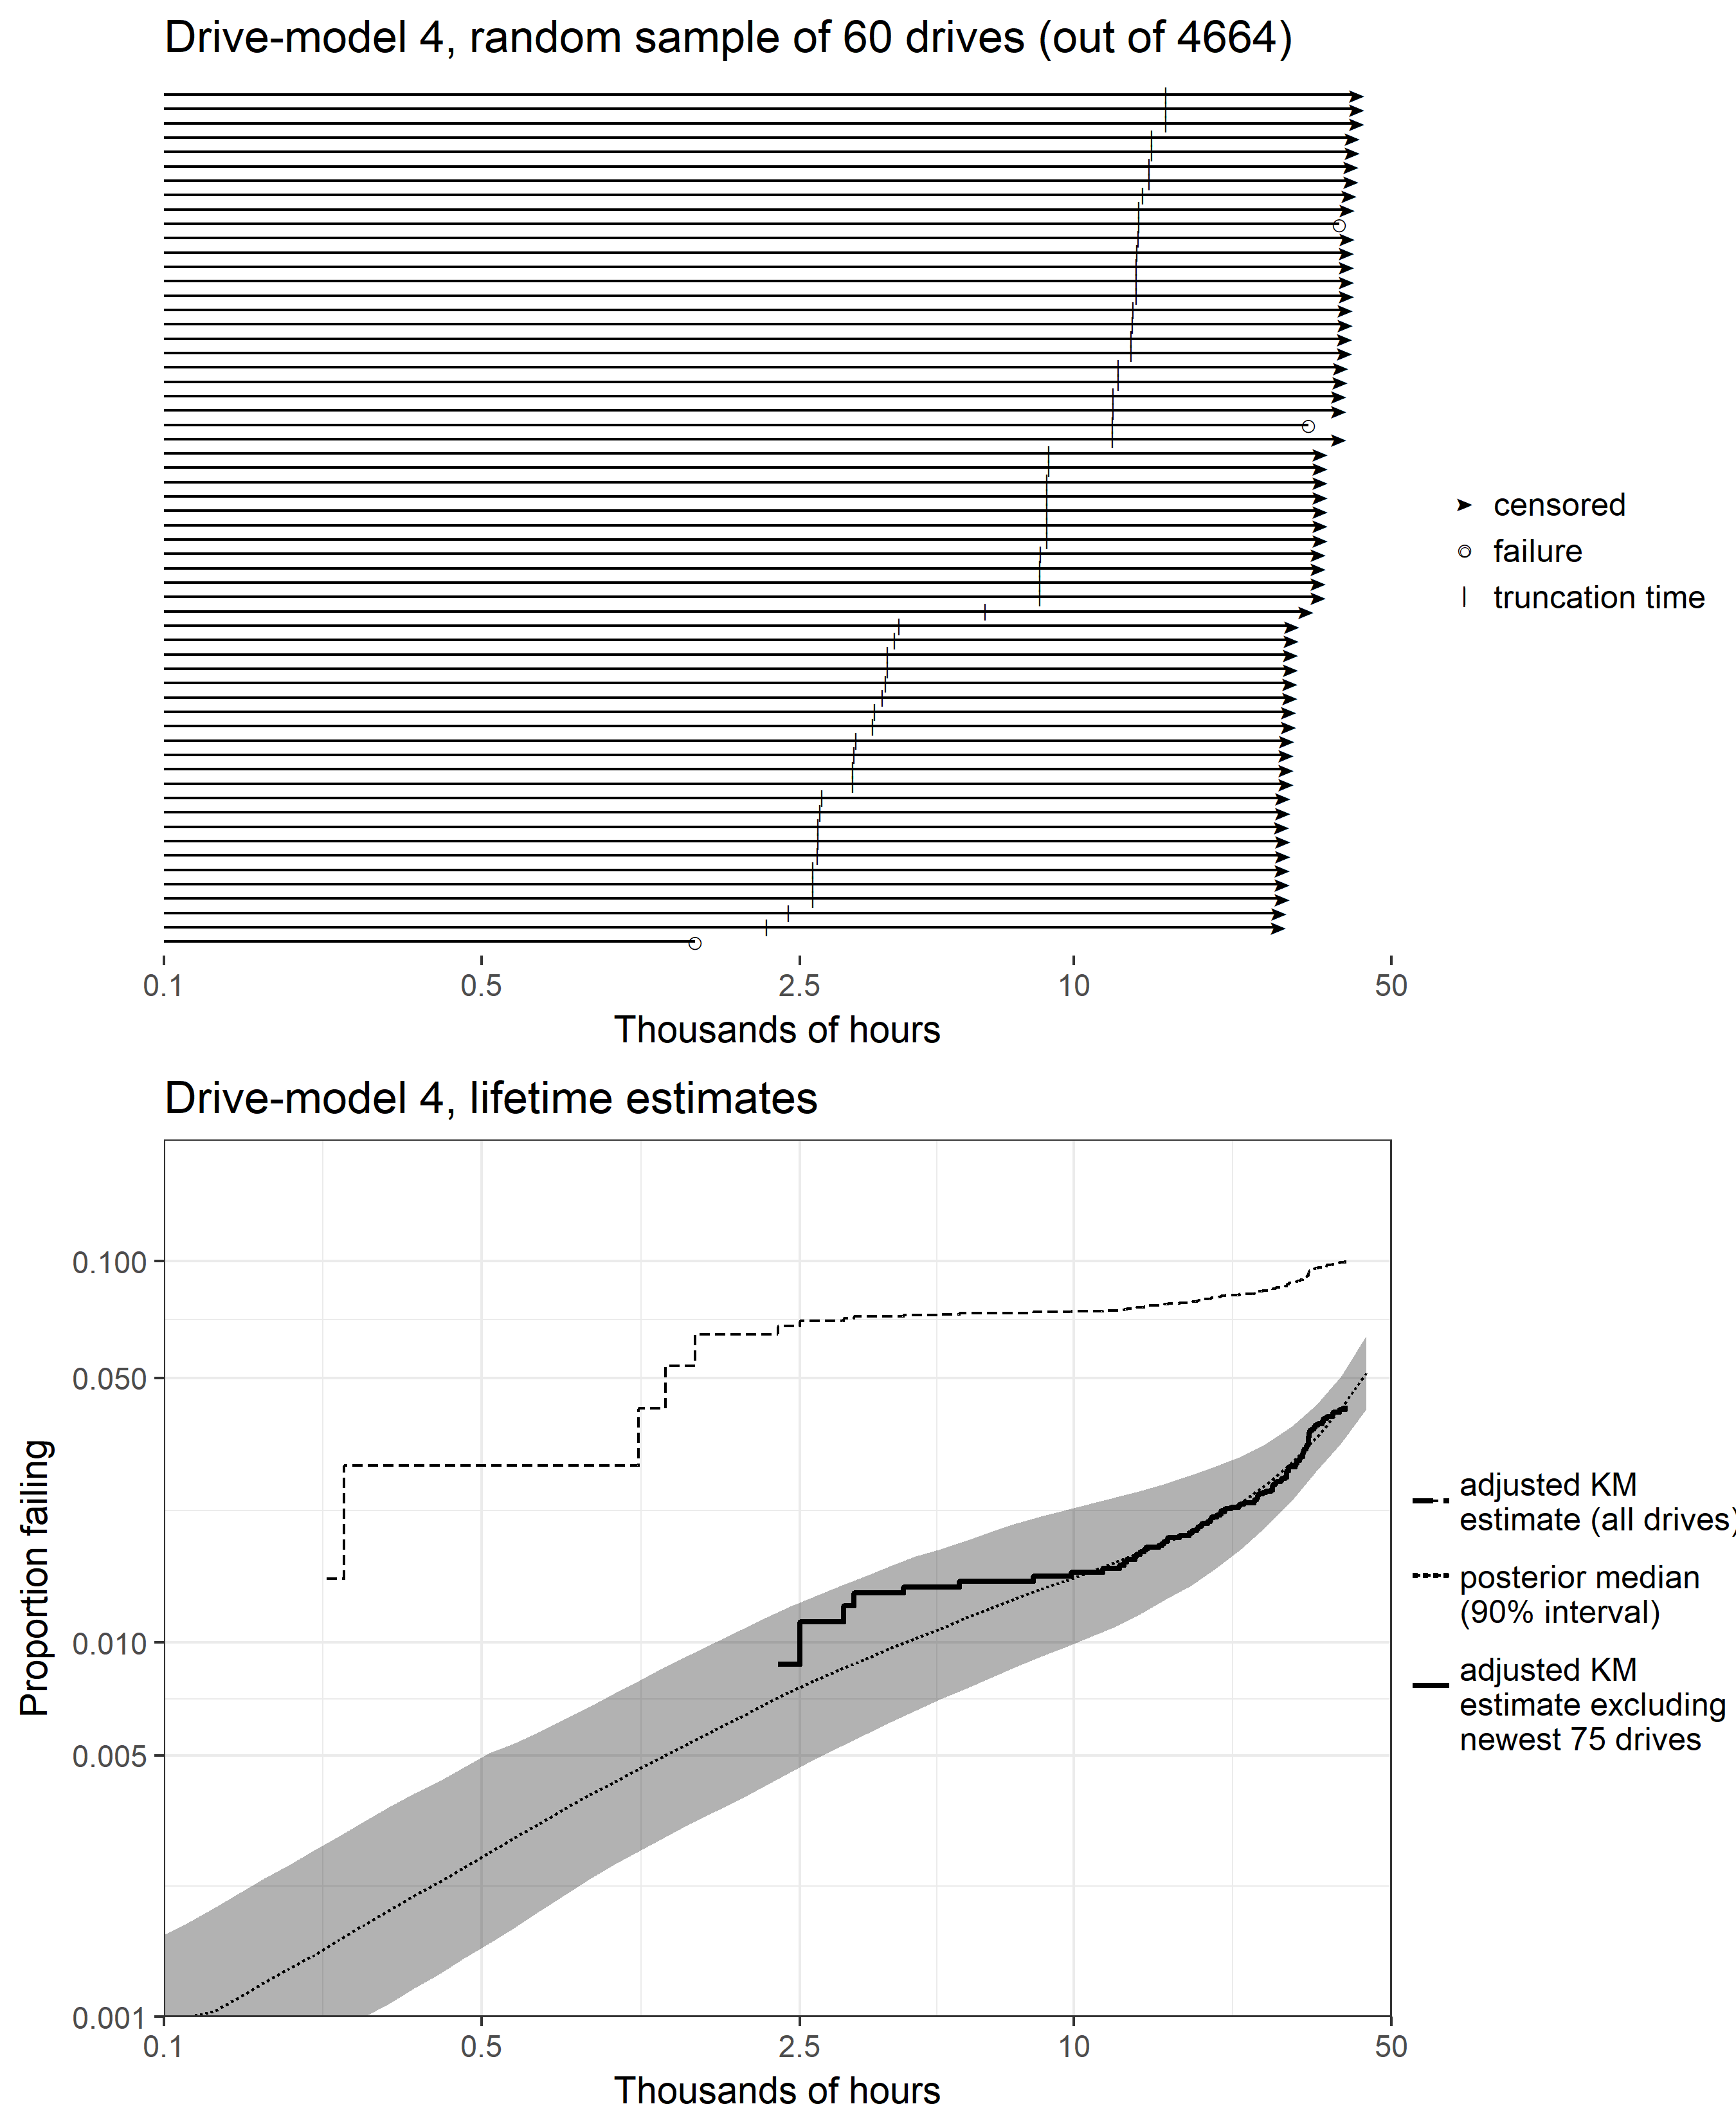
\includegraphics[height=.8\textheight]{dm4-exception.png}
\caption{\footnotesize Top: Event plot for 60 randomly sampled drives of Drive-model 4. Note that all drives in the sample are left truncated well past 1000 hours.\hspace{\textwidth}Bottom: The adjusted K-M estimate (dashed step function) is substantially higher than the pointwise posterior median (dashed line; shaded region showing pointwise 90\% credible intervals). However, this discrepancy is due to several early failures among the small set of drives with the earliest left-truncation times (the newest set). The same adjusted K-M estimator after the exclusion of the newest 75 drives (solid step function) shows close agreement with the posterior median.}

\label{fig:ex-mod-4}
\end{figure}

Figure 8 shows a similar pair of plots for Drive-model 43. The data for this Drive-model are heavily truncated; the observed units had run for quite some time before data were made available with the earliest left-truncation time at 12,189 hours. In the bottom half of Figure \ref{fig:ex-mod-43} we contrast the posterior median for drive-model 43 to an average GLFP cdf for the entire population, which we call the ``global average" cdf; a description of the global average cdf is given in Appendix \ref{global-avg}. We can see that the lack of data for this drive-model during early life results in a diffuse posterior centered around the global average cdf until about 10,000 hours when they diverge. Although the posterior is close to the adjusted K-M, it has been shrunk toward the global average cdf.


\begin{figure}
\centering
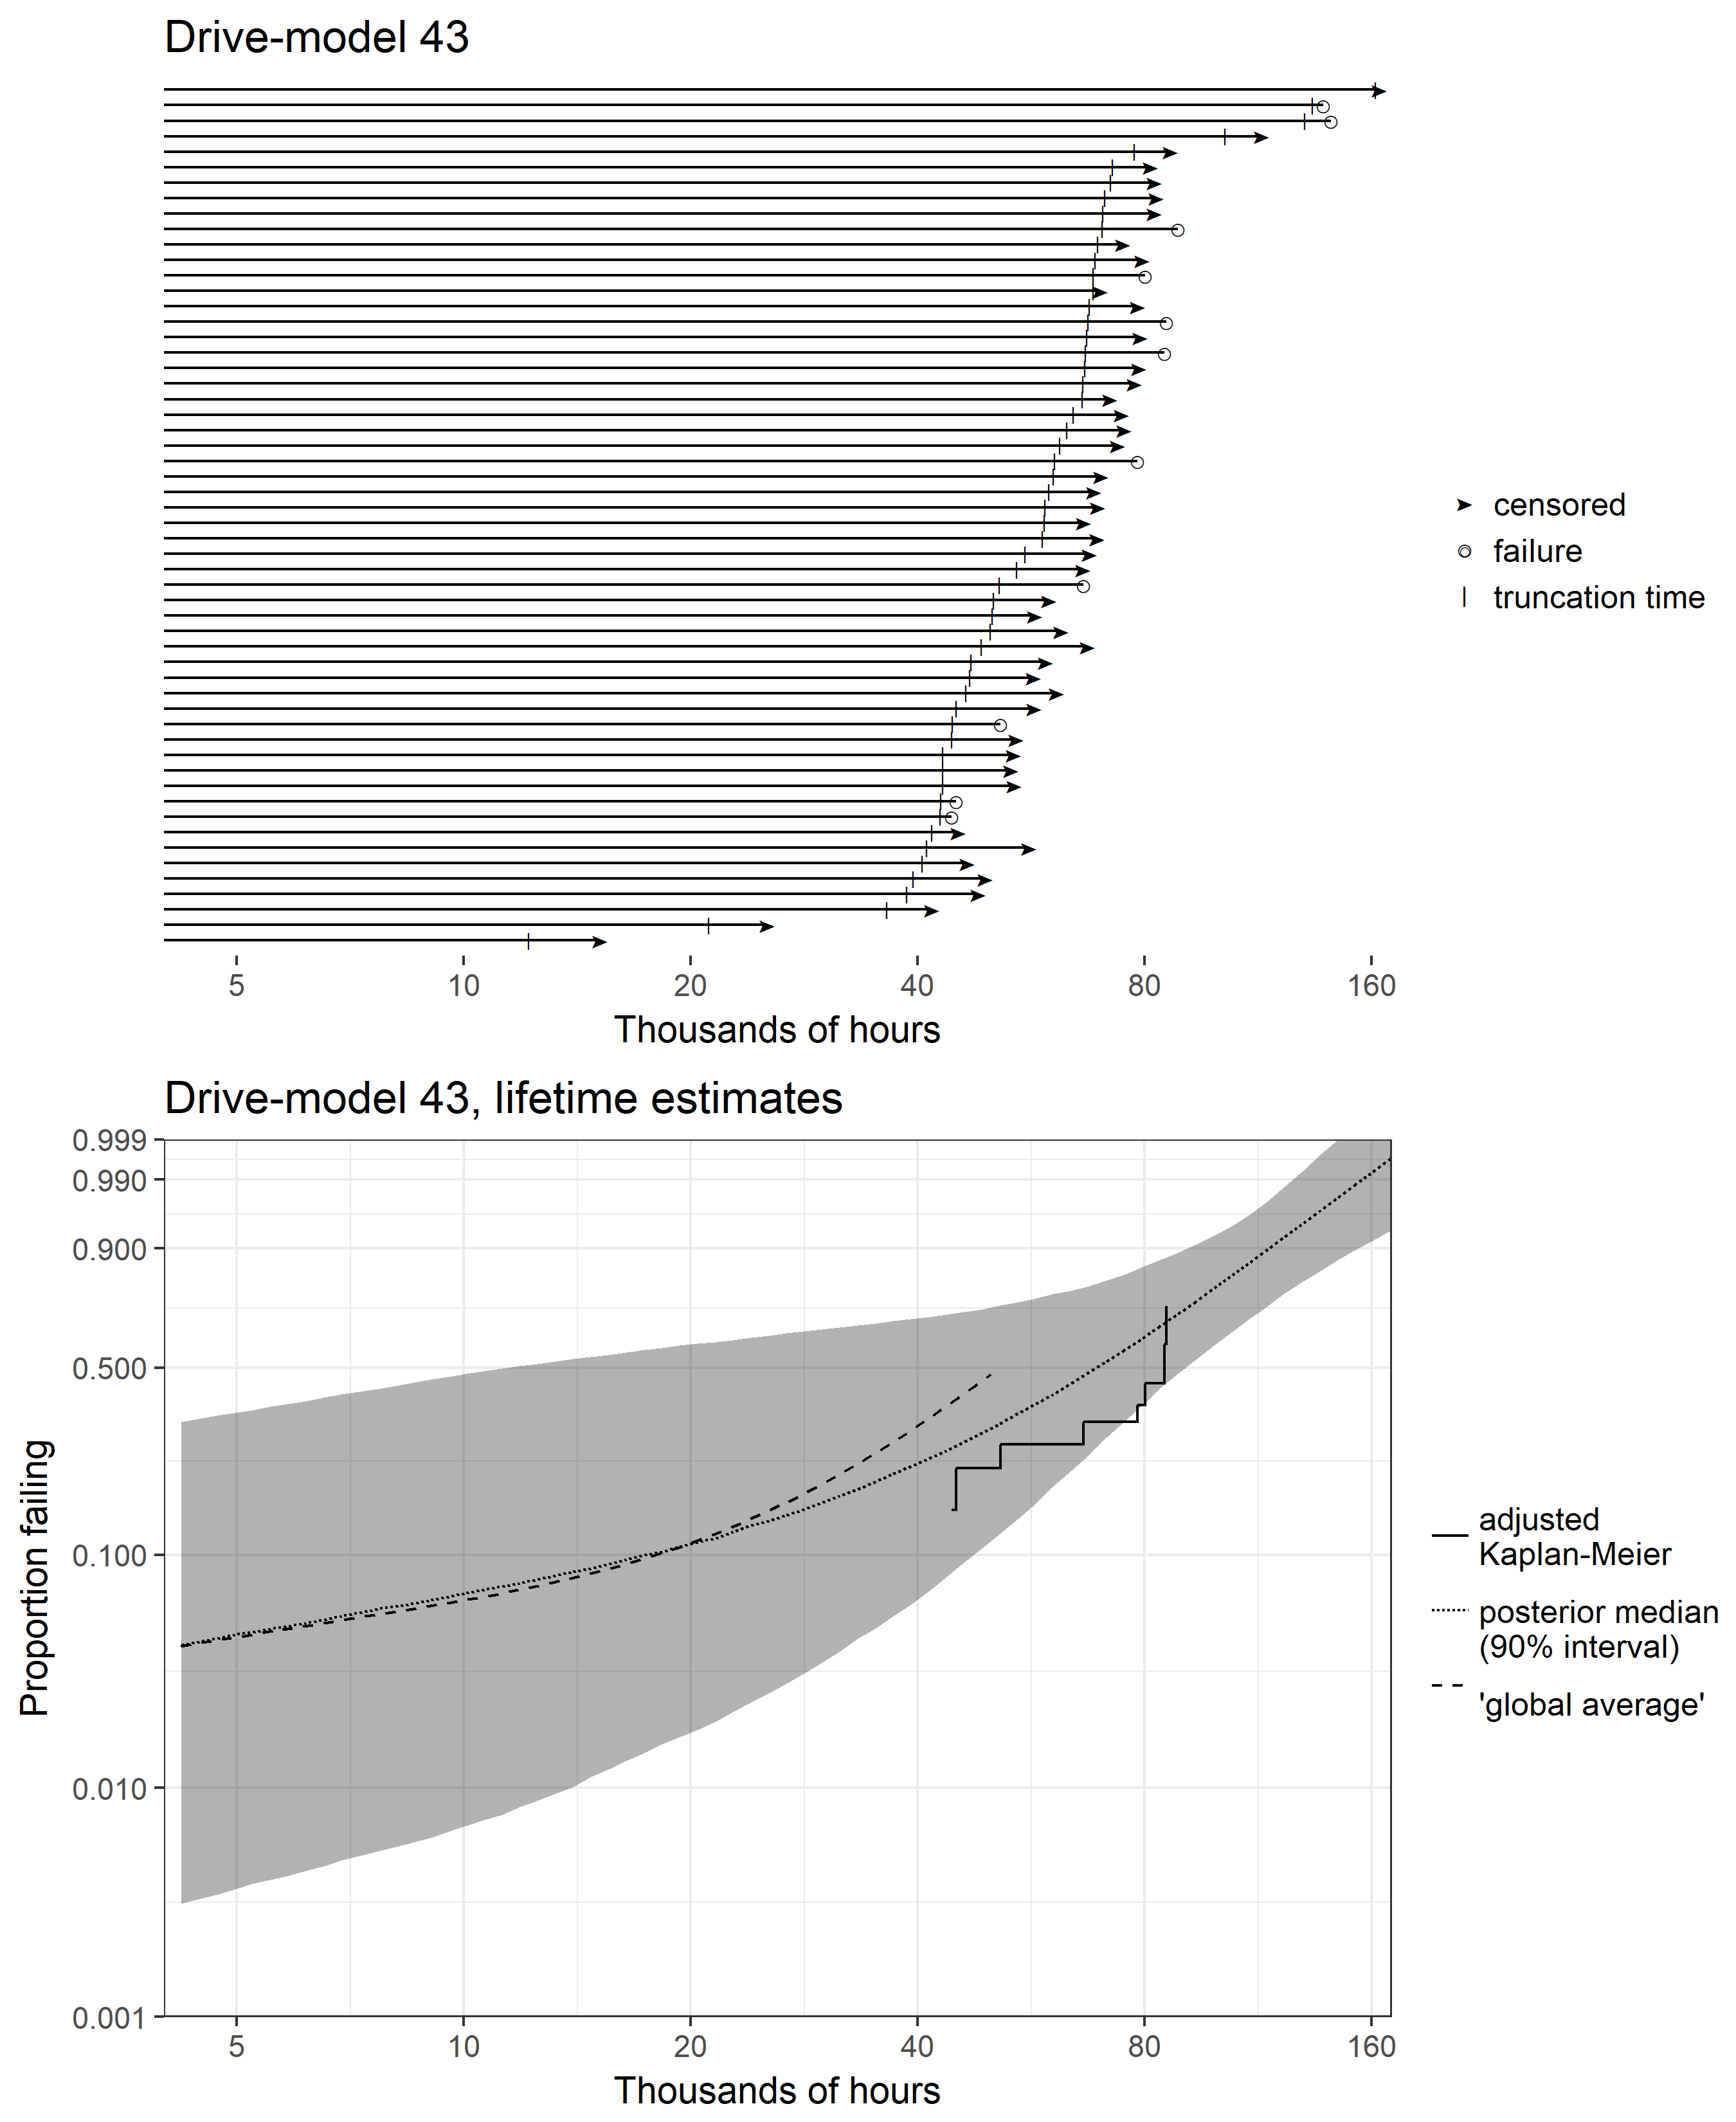
\includegraphics[height=.8\textheight]{dm43-shrinkage.png}
\caption{\footnotesize Top: Event plot for all units of Drive-model 43. Data for all units are left-truncated, being observed conditional on survival beyond 12,000 hours.\hspace{\textwidth}Bottom: The dashed step function correponds to the adjusted K-M estimate (solid line). Due to the heavy left-truncation, the posterior median for Drive-model 43 (dotted line) coincides with the posterior median of the ``global average" (dashed line) until the first left-truncation time.}
\label{fig:ex-mod-43}
\end{figure}

\section{Comparing Sub-populations}
\subsection{Comparisons based on model parameters}
As discussed in Section \ref{sec:Weibull parameterization}, we use a parameterization of the Weibull distribution in terms of a chosen quantile, making prior elicitation straightforward. Posterior sampling immediately gives marginal posterior distributions for quantiles, which in reliability applications is typically more useful than a measure of central tendency. To compare the unconditional $p$ quantile for each sub-population, plots of posterior credible intervals may be used.

Depending on the set of model restrictions used, simlar plots may be used to compare the $p$ quantiles for non-defective units ($t_{p_{2}g}$) or the proportion defective ($\pi_g$).

\subsection{Example: Drive-model comparison based on lower-tail quantiles and proportion defective}
The top panel of Figure 9 shows estimates of $t_{0.10}$ (i.e., the amount of time it takes for 10\% of hard drives to fail, corresponding to the cdf $H(t)$ in Section \ref{subsec:GLFP model}), for all drive-models.  In this application 50\% CIs were used due to considerable posterior uncertainty in some of the parameters: especially for those with few drives in operation.  %Interestingly, the top seven drive-models ranked by MTTF are also the drive-models with the largest $t_{0.10}$.  
The bottom panel of Figure 9 shows the posterior credible intervals for the proportion defective, $\pi_g$, for each drive-model.  The plot is again sorted according to $t_{0.10}$ so it can be compared to the top plot.  While for many of the drive-models the ordinal ranking is the same as on the top, there are some drive-model comparisons, for example 23 and 18, that differ in ranking if compared using $t_{0.10g}$ or $\pi_g$.

\begin{figure}[H]
\centering
   \begin{subfigure}[b]{0.80\textwidth}
   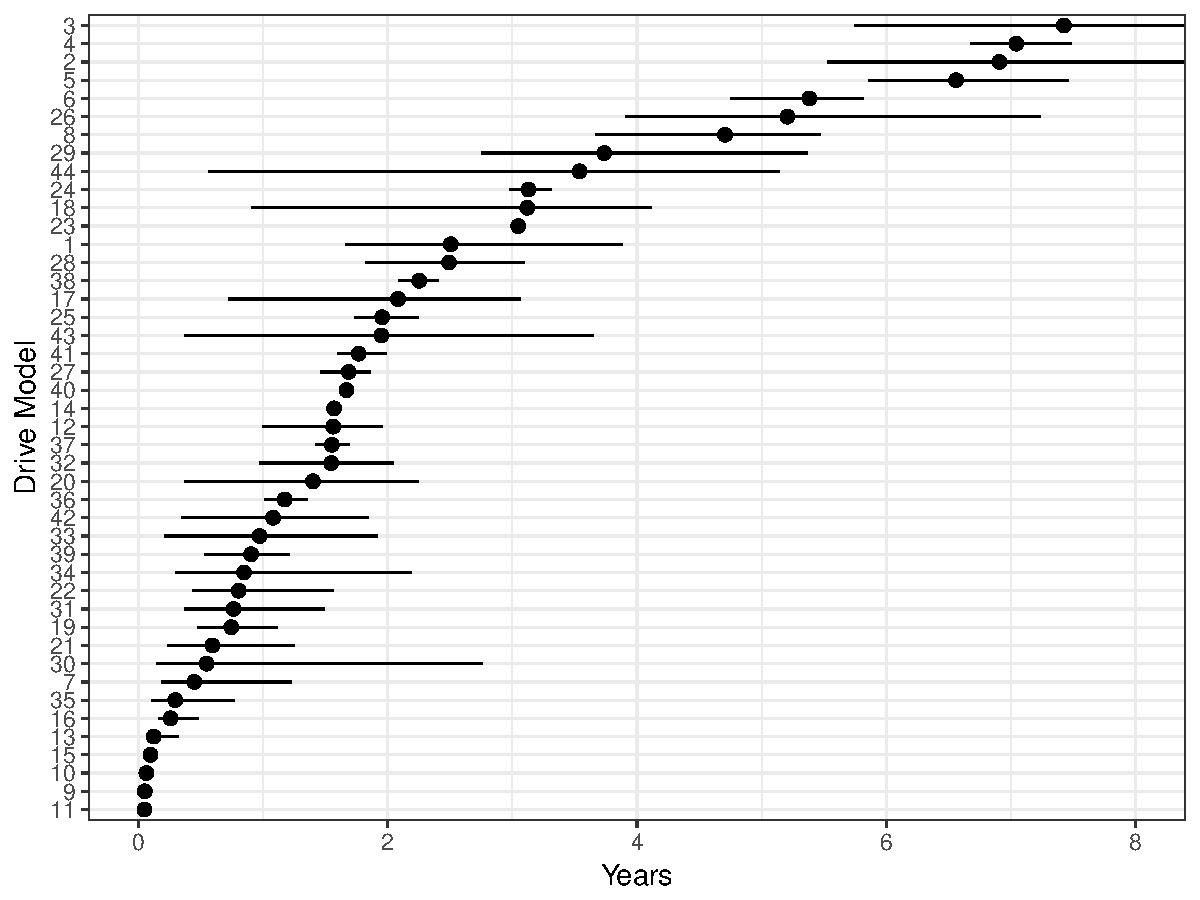
\includegraphics[width=1\linewidth]{b10new.pdf}
   \caption{\footnotesize Point estimate and 50\% CI for $t_{0.10}$}
   \label{fig:Ng1} 
\end{subfigure}

\begin{subfigure}[b]{0.80\textwidth}
   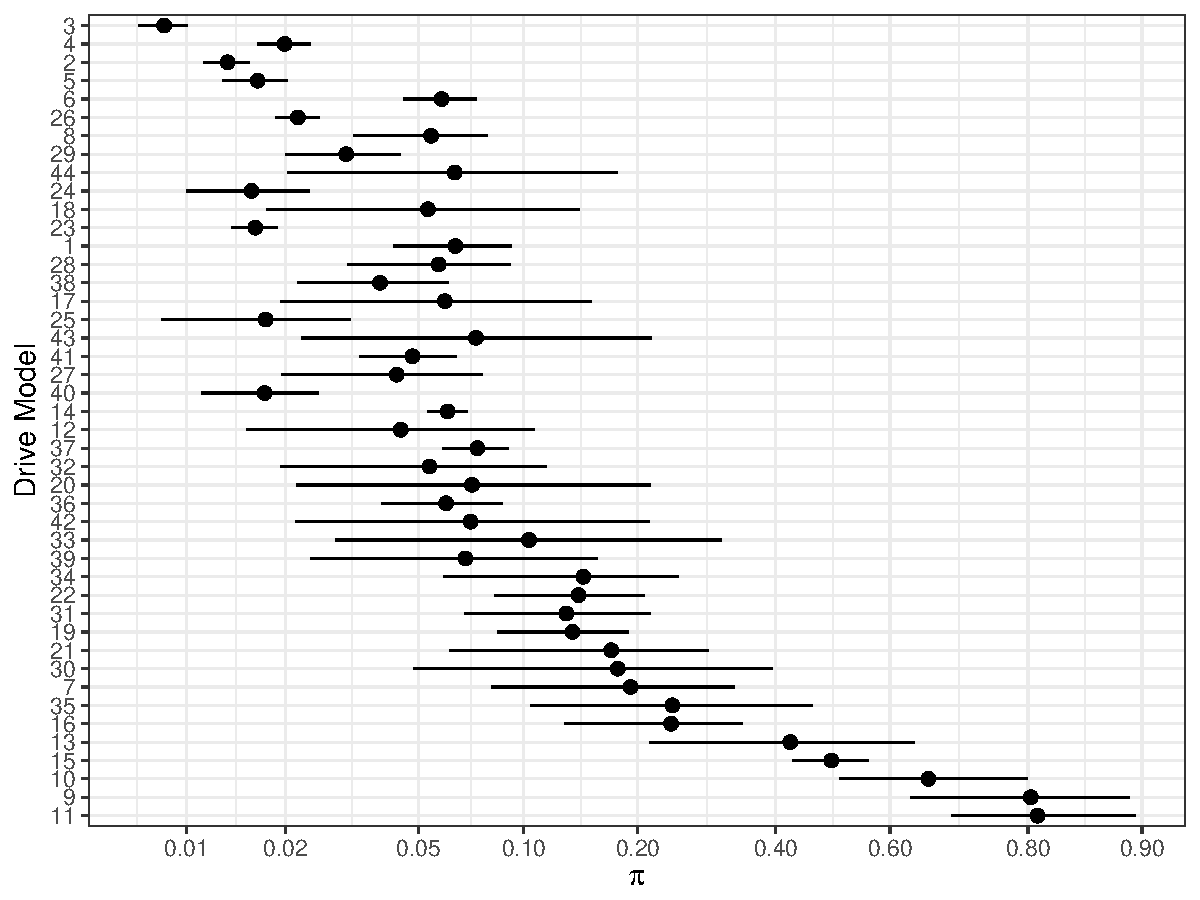
\includegraphics[width=1\linewidth]{pinew.pdf}
   \caption{\footnotesize Point estimate and 50\% CI for $\pi$}
   \label{fig:Ng2}
\end{subfigure}

\caption{\footnotesize (a) 50\% CI (in years) for $t_{0.10}$ (b) 50\% CI for $\pi$ plotted on the logit scale.  Both plots are sorted based on the median value of the marginal posterior distribution of $t_{0.10}$.}
\end{figure}

 
 
%\begin{figure}[H]
  %\centering
  %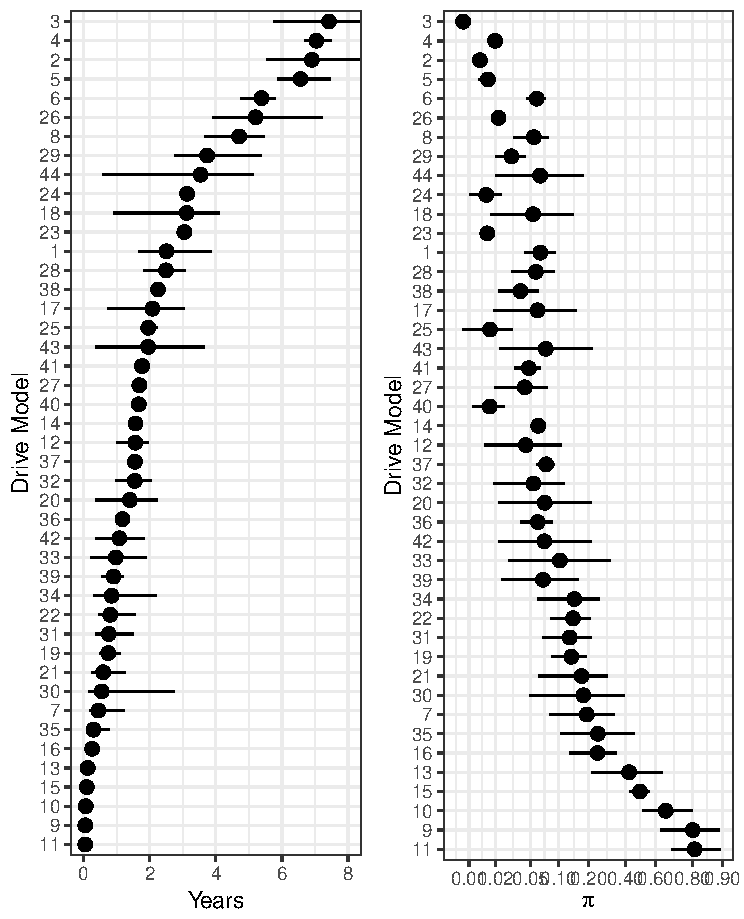
\includegraphics[width=\textwidth]{b10andpi}
  %\caption{Left: 50\% credible intervals for  $t_{0.10}$ (time in years till 10\% of the drives fail). Right: 50\% credible intervals for $\pi$ plotted on the logit scale.  Both plots are sorted based on the median value of $t_{0.10}$.}
  %\label{fig4}
%\end{figure}



\subsection{Comparisons based on posterior predictive distribution}
By utilizing samples from the full posterior distribution, in addition to estimation of the model parameters, we can also produce forecasts for new units or groups of units. In many situations, this may more directly address issues of importance.

The {\em posterior predictive} distribution incorporates two sources of variability: the posterior uncertainty in the parameters, which largely depends on the
amount of data collected, and the uncertainty in future
observations conditional on those parameters. 

For example,
\begin{equation*}
  p(t_{g,new}|t) = \int p(t_{g,new}|\theta_g) p(\theta_g|t_g) \, d\theta_g
\end{equation*}
gives the posterior predictive density for a new unit from sub-population $g$.

We can sample from this distribution by drawing $t_{g,new}^{(s)}$ from
$\operatorname{GLFP}(\pi_g^{(s)},
t_{p1}^{(s)},\sigma_1^{(s)},t_{p_{2}g}^{(s)},\sigma_{2g}^{(s)})$, for
$s=1,...,S$, using the saved posterior draws for the model
parameters. 

\begin{figure}[H]
  \centering
  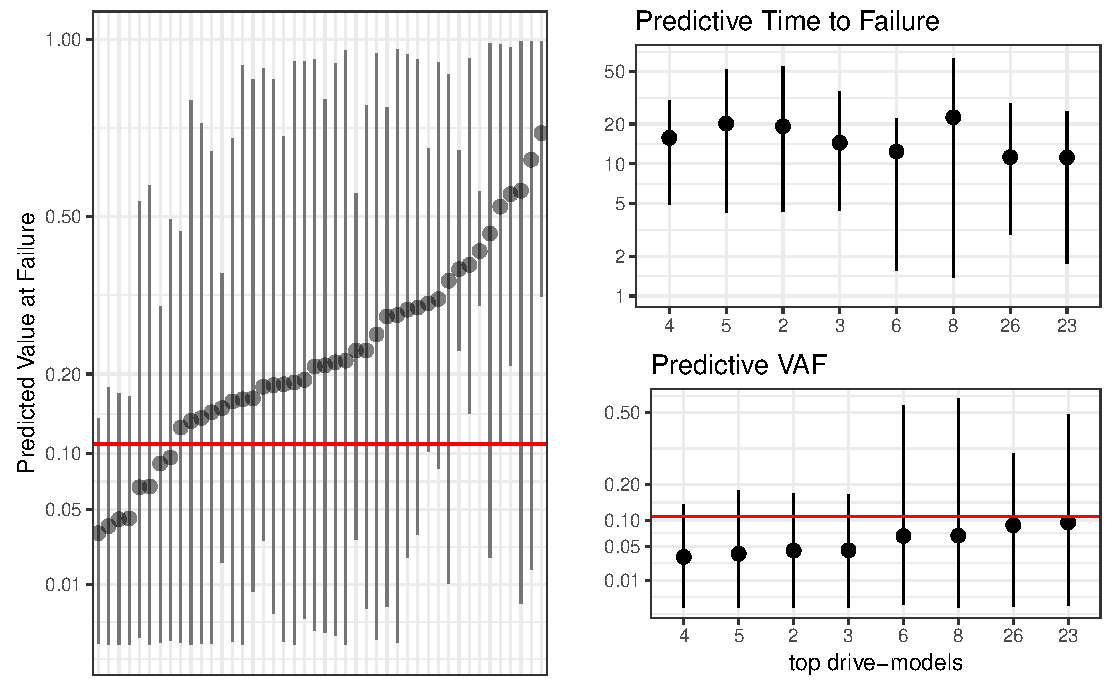
\includegraphics[width=.8\textwidth]{dm-eval}
  \caption{\footnotesize Left: 90\% CI of the posterior predictive distributions for $e^{-0.4 t_{g,new}}$ the depreciated value at failure (VAF) for a new unit for each Drive-model.
  Right: A comparison (90\% CI) of the predictive distribution of TTF in hundreds of thousands of hours (top) and VAF (bottom) based on 40\% depreciation for the best 11 drive-models, shows that rankings produced by the two measures are not equivalent.}
  \label{fig5}
\end{figure}

\subsection{Example: Drive-model comparison based on predictive distribution of new unit}

Here we show how to rank drive-models with respect to economical value. From a
business perspective, it is clear
that we should prefer drive-models that will provide more years
of service. For ease of exposition, we will assume that the purchase
price of a hard-drive is the same across drive-models.

The mean time-to-failure (MTTF) for drive-model $d$ can be estimated by
$$\frac{1}{S} \sum_{s=1}^{S} t_{g,new}^{(s)}.$$
where $t_{g,new}^{(s)}$ is a draw from the posterior predictive distribution for drive-model $g$. 

While MTTF is often an important metric, due to the
anticipation of advancements in technology, we can expect that the
relative value of computer hardware will depreciate rather quickly. In simple terms, given two hard drives, one would prefer to have both of them work for five years than for one to work for nine years and the other to work for just one year. To account
for depreciation, rather than using MTTF as the metric for drive-model comparison, we use the value at replacement. The US Internal Revenue Service considers
computer hardware to be ``5-year'' equipment \citep{f4562}. Using``the declining
balance method'' the rate of depreciation is 40\% per year.

Let $L(t) = e^{-0.4t}$ represent the value at the time of failure
relative to a new unit. We can rank the drive-models by 
$$\op{E}(L(t_{g,new})|t))\approx \frac{1}{S} \sum_{s=1}^{S} L(t_{g,new}^{(s)}).$$

Posterior credible intervals for $L(t_{g,new})$ are shown in the left panel of Figure \ref{fig5}. A zoomed version for the top eight drive-models, as ranked by $\op{E}(L(t_{g,new})|y)$ are shown in the bottom right panel. The panel above shows credible intervals for MTTF. We can see that ranking by MTTF would lead to a different result -- a new Drive-model 8 unit is expected to last the longest, but the possibility of it failing early is higher than for the drive-models ranked highest by our depreciation-aware metric. The top four drive-models (4, 5, 2, 3) are comparable, with a new Drive-model 4 unit expected to depreciate the most. However, given the discrepancy of the model fit for Drive-model 4 (noted in the previous subsection), in the absence of more early life data, we might harbor some lingering concern about possible quality-control issues with this Drive-model.




\section{Discussion}
\label{sec:Discussion}
This paper offers a new approach to modeling and making inference for the lifetime of consumer products using incomplete field reliability data.  Products with long lifetimes often have few failures and when failures do occur the cause is frequently unknown to the analyst.  The GLFP model provides a framework to accurately model data with evidence of multiple failure modes that behave differently (e.g., early failures and wearout failures). Moreover, when there are multiple product populations within the same product class, our hierarchical modeling approach borrows strength across brands with many observed failures to help make inference for those brands with few failures.  This can be important when trying to leverage multiple sources of data with various sample sizes and levels of censoring and truncation.

In the case of the Backblaze data, we observed improved posterior precision for quantities of interest when using our hierarchical model when compared to separate models for lifetime by drive-model. This is illustrated in Figure \ref{improved_accuracy}. In addition, this leveraging information led to well-behaved posterior distributions for sub-populations with few observed failures. For many of these sub-populations, fitting separate GLFP models was unworkable.

\begin{figure}
  \centering
  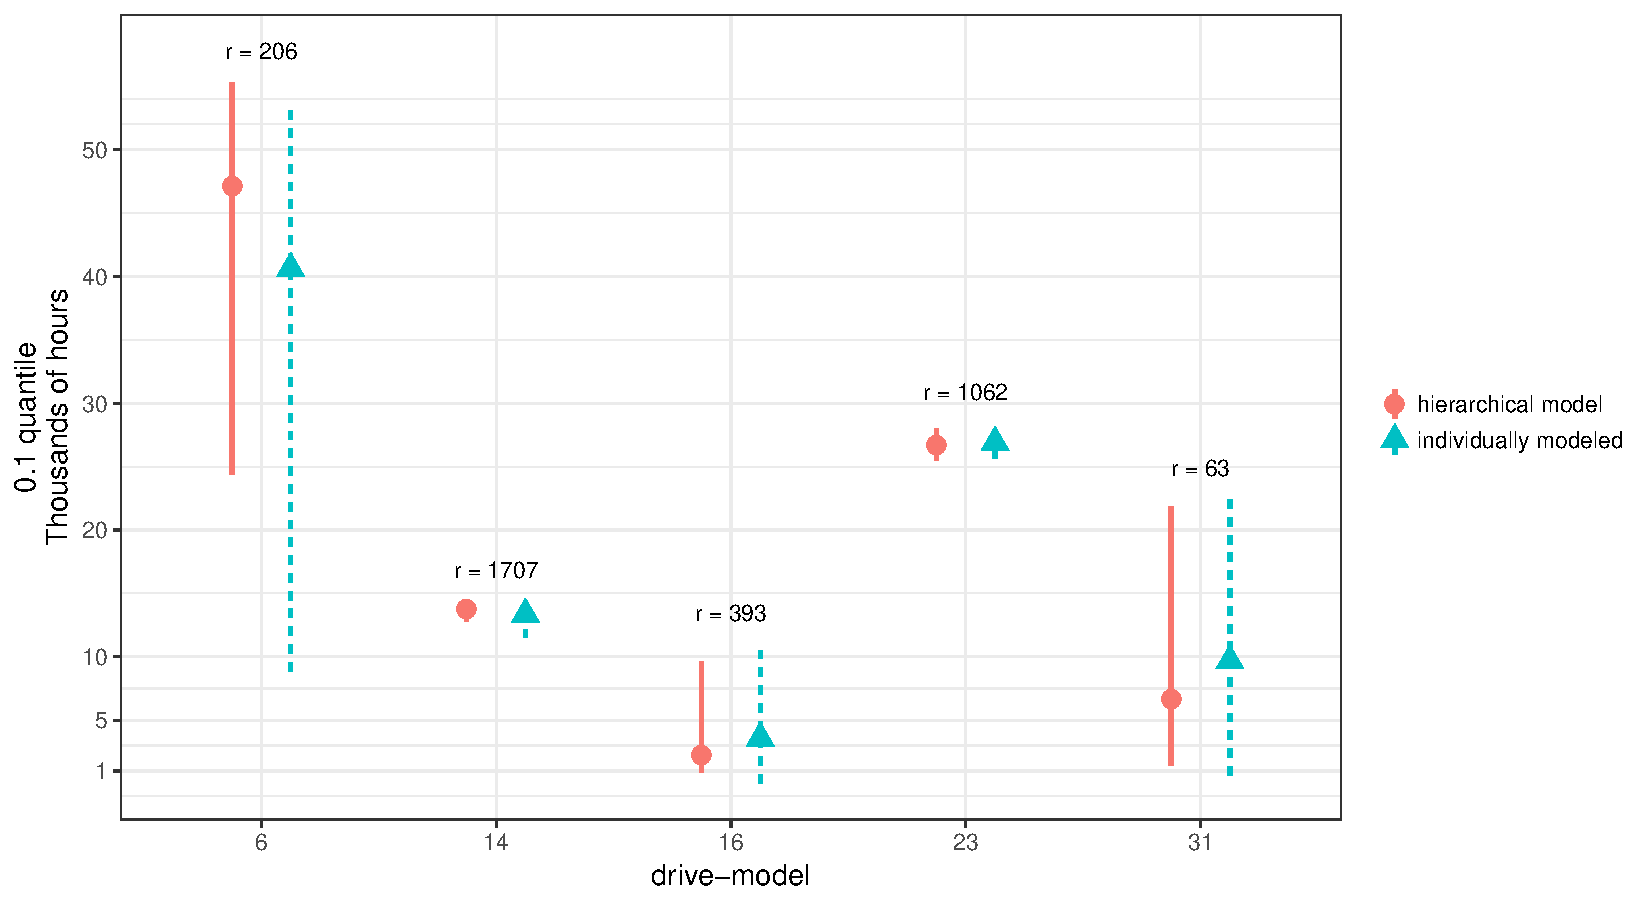
\includegraphics[width=.7\textwidth]{accuracy_compare}
  \caption{\footnotesize Posterior distributions of 0.1 quantiles for a representative subset of drive-models where separate fitting of the GLFP model was successful (unimodal posteriors and passing MCMC convergence diagnostics.) $r$ indicates the number of observed failures. Separate fits use the same priors as Model 4, but have greater uncertainty because there is no borrowing of information across drive-models.}
  
\label{improved_accuracy}
\end{figure}

We now address some important model assumptions and their potential for impacting statistical inference. 

First, we assume the failures occurring from various causes can be approximately assigned to two phases of product life.  In practice, there might be additional phases, clearly supported by the data, making the GLFP model too rigid. This rigidity is illustrated by the right tail of the estimated distribution in Figure \ref{fig1}.

Second, we assume exchangability of units within a sub-population. This assumption is due in part to ignorance about which units are defective but also of potentially important covariates. We do not account for batch effects or varying conditions in the facility which have impacted the observed failure rates. These factors are confounded with drive-model in our analysis. An example of a possible batch effect is noted in Section \ref{model-assessment} and illustrated by Figure \ref{fig:ex-mod-4}. 

Consumers of manufactured products usually lack the data, expertise, or motivation to perform a failure analysis to determine the cause of failure.  Their interest is primarily in the lifetime distribution of a product rather than the specific cause of failure.  The ability to fit marginal models, such as GLFP, allow consumers and manufacturers to accurately model products with bathtub hazard lifetime distributions and make comparisons across different product sub-populations.  Because the Bayesian approach provides full posterior distributions once a model is fit, the analyst can easily estimate a functional, such as a quantile or depreciation factor, that allow products to be compared using statistics that are meaningful in the context of the actual application. 

While not presented here, another potential application is forecasting the number of future failures over a fixed period of time for a current population of drives. \citet{hmm} proposed a method, based on the Poisson-binomial distribution. It would be straightforward to adapt their approach to work with our method. For details and examples see \citet[Sect.~6]{hmm} and \citet{xu2015assessing}.

\section*{Acknowledgment}    
The authors express their gratitude to Nick Clark for his helpful comments and suggestions.  We would also like to thank the anonymous referees who provided 
many useful suggestions that helped improve this paper.

%Hierarchical modeling can be an effective way to regularize a large number of models fits by borrowing information.  %Because all the data contribute some information about the global parameters, it is often sufficient to use weakly %informative priors on the global parameters, making the resulting shrinkage data dependent.  Analysis using HMC is %accessible to practitioners by Stan. HMC has been shown to be very efficient in effective samples per iteration because %its joint updating scheme.  
\clearpage

\appendix
\section{Truncation adjusted Kaplan-Meier estimate of lifetime}
\label{sec:trunc-adj}
We first start with a nonparametric estimate of the empirical cdf for each sub-population using the Kaplan-Meier estimator.  With left truncation, however, the standard Kaplan-Meier estimator for drive-model $g$, denoted by
$\widehat{F_g(t)}_{KM}$, is conditional on survival up to
$t_{g,\text{min}}^L$, the shortest reported running time of all units in
of sub-population $g$ for which records are available. To produce
unconditional estimates, we adapt the adjustment method outlined by \citet[Chapter 11]{meeker}.  For each sub-population we select
$t_{g,\text{min}}^L$, the smallest left truncated time in the sample.
By sampling from the full posterior distribution, because
$\Pr(T>t_{g,\text{min}}^L|\theta_g)$ (the probability that a hard drive has
survived up to $t_{g,\text{min}}^L$) is a function of the model
parameters, we can easily compute its posterior median,
$\widehat{A}_{\text{med}} = \widehat{\Pr}(T>t_{g,\text{min}}^L|\theta_g)$. We compute the adjusted estimate by

$$\widehat{F(t)}_{KMadj} = \widehat{A}_{\text{med}} + \left(1 - \widehat{A}_{\text{med}}\right)\widehat{F_g(t)}_{KM},\; t>t_{g,\text{min}}^L.$$

While this adjustment may be negligible for sub-populations with little truncation, in our Backblaze example, five drive-models receive upward adjustments of greater than 5 percent and the estimated time to failure distribution of one drive-model (30) was adjusted by nearly 16 percent, in part because the shortest truncation time for all observed units was approx. 2.3 years.

\section{Definition of global average for Model 4}
\label{global-avg}
In Section \ref{model-assessment}, to illustrate the concept of shrinkage in our hierarchical model, we refer to a ``global average" which represents an average GLFP cdf for the entire population, $\op{H}\left(\cdot|\bar{\pi},\mu_1,\sigma_1,\bar{\mu}_2,\bar{\sigma}_2\right)$. Because $\mu_1$ and $\sigma_1$ are common across all sub-populations in our model, these can already be interpreted as ``global." For the parameters that vary across sub-populations, we select values corresponding to the medians of the hierarchical distributions (\ref{eq:hier-model}) conditional on the hyperparameters. In particular, we set
$$\bar{\pi}=\op{logit}^{-1}(\eta_{\pi}),\;\bar{\mu}_2=\eta_{t_2} - m_{\sigma_2}\Phi^{-1}(.2) \mbox{ and } \bar{\sigma}_2= m_{\sigma_2}.$$
Let $J(\cdot|a,b),\;J^{-1}(\cdot|a,b)$ denote the cdf and inverse cdf, respectively, for a lognormal distribution with log-location parameter $a$ and log-scale parameter $b$. Then
$$m_{\sigma_2}=J^{-1}[0.5 \cdot J(1|\eta_{\sigma_2},\tau_{\sigma_2})|\eta_{\sigma_2}, \tau_{\sigma_2}],$$
which is the median of a lognormal distribution with parameters $\eta_{\sigma_2}$, and $\tau_{\sigma_2}$, truncated to the interval $(0, 1)$.

We estimate the global average pointwise, using draws from the joint posterior distribution, $H\left(\tilde{t}|\eta_\pi^{(s)}, \mu_1^{(s)}, \sigma_1^{(s)}, \eta_{t_2}^{(s)},\eta_{\sigma_2}^{(s)},\tau_{\sigma_2}^{(s)}\right)$, $s=1,2,\ldots,S$. The computation is thus similar to that shown in (\ref{pointwise-medians}).
 % We get this by setting the $\op{GLFP}$ parameters equal to the median of their hierarchical distribution, i.e., $\pi=\op{logit}^{-1}(\eta_{\pi}^{(s)}),\, \mu_1=\mu_1^{(s)},\, \sigma_1=\sigma_1^{(s)},\, \mu_2=\eta_{t_2}^{(s)} - m_{\sigma_2}^{(s)} \Phi_{SEV}^{-1}(.2)$ and $\sigma_2= m_{\sigma_2}^{(s)}$, where $m_{\sigma_2}^{(s)}=F^{-1}[0.5 \cdot F(1;\eta_{\sigma_2}^{(s)},\tau_{\sigma_2}^{(s)});\eta_{\sigma_2}^{(s)}, \tau_{\sigma_2}^{(s)}]$ is the population median of the $\sigma_{2g}$, conditioning on $\left(\eta_{\sigma_2}^{(s)},\tau_{\sigma_2}^{(s)}\right)$. The curve was estimated using pointwise medians as in Equation \ref{pointwise-medians}.


\section{Supplementary Material}
\label{sec:supple}

\begin{description}

\item[Model code and plots] Stan code for Model 4 as well as the complete set of plots similar to Figures 5 and 6 (supplementary.pdf)

\item[Backblaze data set] Lifetime data set for all 44 Backblaze drive-models used in our analysis. (backblaze\_hd\_data.csv)

\end{description}

%\begin{supplement}
  %\sname{Supplement A}
  %\stitle{Stan Code and Plots}
  %%\slink[doi]{COMPLETED BY THE TYPESETTER}
  %\sdatatype{.pdf}
  %\sdescription{Stan code for Model 4 as well as the complete set of plots for Figures 5 and 6.}
%\end{supplement}
%
%\begin{supplement}[id=suppB]
  %\sname{Supplement B}
  %\stitle{Backblaze Data}
  %\slink[doi]{COMPLETED BY THE TYPESETTER}
  %\sdatatype{.csv}
  %\sdescription{Lifetime data set for all 44 drive-models used in our analysis.}
%\end{supplement}


\bibliography{./sample}

% AOS,AOAS: If there are supplements please fill:
%\begin{supplement}[id=suppA]
%  \sname{Supplement A}
%  \stitle{Title}
%  \slink[doi]{10.1214/00-AOASXXXXSUPP}
%  \sdatatype{.pdf}" 
%  \sdescription{Some text}
%\end{supplement}


\end{document}
